\documentclass[11pt,a4paper,twoside]{book}
\usepackage[T1]{fontenc}
\usepackage[utf8]{inputenc}
\usepackage{mathpazo}
\usepackage[scaled=0.90]{helvet}
\usepackage{courier}
\usepackage[a4paper,inner=3.0cm,outer=2.4cm,top=2.6cm,bottom=2.8cm]{geometry}
\usepackage{xcolor}
\usepackage{mathtools}
\usepackage{colortbl}
\usepackage{tikz}
\usetikzlibrary{calc,positioning,arrows.meta,decorations.pathmorphing}
\usepackage{booktabs}
\usepackage{array}
\usepackage{longtable}
\usepackage{enumitem}
\usepackage[german=quotes]{csquotes}
\usepackage{fancyhdr}
\usepackage{titlesec}
\usepackage{amsmath,amssymb}
\usepackage{tcolorbox}
\tcbuselibrary{skins,breakable}
\usepackage[hidelinks]{hyperref}

\definecolor{tief}{HTML}{1F3A5F}
\definecolor{mittel}{HTML}{2E5F8A}
\definecolor{akzent}{HTML}{A34A28}
\definecolor{sand}{HTML}{F4F1EA}
\definecolor{grau}{HTML}{5A5A5A}
\definecolor{gruen}{HTML}{2F6B4F}
\definecolor{purpur}{HTML}{5B3A72}

\newcolumntype{P}[1]{>{\raggedright\arraybackslash}p{#1}}

\newcommand{\kursiv}[1]{{\itshape\color{grau}#1}}
\newcommand{\code}[1]{{\ttfamily\small #1}}
\newcommand{\Person}[1]{\textbf{#1}}
\newcommand{\Begriff}[1]{\textbf{#1}}
\newcommand{\zit}[1]{\textsuperscript{[#1]}}
\newcommand{\Oh}{\mathcal{O}}
\newcommand{\boxtitel}[1]{{\bfseries\color{tief}#1}\par\vspace{6pt}}
\newcommand{\boxtitelr}[1]{{\bfseries\color{akzent}#1}\par\vspace{6pt}}
\newcommand{\boxtitelg}[1]{{\bfseries\color{gruen}#1}\par\vspace{6pt}}
\newcommand{\boxtitelp}[1]{{\bfseries\color{purpur}#1}\par\vspace{6pt}}
\newcommand{\boxtitelm}[1]{{\bfseries\color{mittel}#1}\par\vspace{6pt}}
\newcommand{\loesung}{\par\vspace{8pt}{\bfseries\color{mittel}Lösung}\par\vspace{4pt}}
\newcommand{\schritt}[1]{\par\vspace{5pt}{\bfseries\color{grau}#1}\par\vspace{2pt}}

% Graphentheoretische Notation
\newcommand{\Gr}{G}
\newcommand{\Kn}[1]{K_{#1}}
\newcommand{\Kmn}[2]{K_{#1,#2}}
\newcommand{\Grad}{\deg}
\newcommand{\Nb}{N}
\newcommand{\chrom}{\chi}
\newcommand{\Ecken}{V}
\newcommand{\Kanten}{E}

\newtcolorbox{grundbox}[1][tief]{
  breakable, enhanced, colback=sand, colframe=sand,
  boxrule=0pt, leftrule=3pt, borderline west={3pt}{0pt}{#1},
  left=12pt, right=10pt, top=10pt, bottom=10pt,
  sharp corners, before skip=12pt, after skip=12pt}

\newenvironment{merksatz}{\begin{grundbox}[tief]}{\end{grundbox}}
\newenvironment{warnung}{\begin{grundbox}[akzent]}{\end{grundbox}}
\newenvironment{definition}{\begin{grundbox}[mittel]}{\end{grundbox}}
\newenvironment{geschichte}{\begin{grundbox}[gruen]}{\end{grundbox}}
\newenvironment{forschung}{\begin{grundbox}[purpur]}{\end{grundbox}}
\newenvironment{aufgabe}{\begin{grundbox}[grau]}{\end{grundbox}}
\newenvironment{technik}{\begin{grundbox}[mittel]}{\end{grundbox}}

\titleformat{\chapter}[display]
  {\normalfont\huge\bfseries\color{tief}}{\Large\color{grau}Kapitel \thechapter}{8pt}{\Huge}
\titleformat{\part}[display]
  {\normalfont\huge\bfseries\color{tief}\filcenter}{\Large\color{grau}Teil \thepart}{10pt}{\Huge}
\titlespacing*{\chapter}{0pt}{10pt}{28pt}

\pagestyle{fancy}
\fancyhf{}
\fancyhead[LE,LO]{\small\itshape\color{grau}\leftmark}
\fancyfoot[LE,LO]{\small\color{grau}\thepage}
\renewcommand{\headrulewidth}{0.4pt}
\renewcommand{\footrulewidth}{0pt}
\renewcommand{\chaptermark}[1]{\markboth{#1}{}}
\setlength{\parindent}{0pt}
\setlength{\parskip}{6pt}
\renewcommand{\arraystretch}{1.3}

\renewcommand{\contentsname}{Inhaltsverzeichnis}
\renewcommand{\chaptername}{Kapitel}
\renewcommand{\partname}{Teil}
\renewcommand{\appendixname}{Anhang}
\renewcommand{\tablename}{Tabelle}
\renewcommand{\figurename}{Abbildung}

\hyphenation{Spiel-the-o-rie spiel-the-o-re-tisch Aus-zah-lung Aus-zah-lungs-ma-trix
Stra-te-gie Stra-te-gi-en Stra-te-gie-raum
Gleich-ge-wicht Gleich-ge-wich-te Nash-Gleich-ge-wicht Sat-tel-punkt
Mi-ni-max Ma-xi-min Null-sum-men-spiel Nicht-null-sum-men-spiel
Do-mi-nanz do-mi-niert Do-mi-nanz-eli-mi-na-ti-on
Ge-fan-ge-nen-di-lem-ma Ko-or-di-na-ti-ons-spiel
Nor-mal-form ex-ten-si-ve Rück-wärts-in-duk-ti-on Teil-spiel
Wie-der-ho-lung Ver-gel-tungs-stra-te-gie
evo-lu-ti-o-när evo-lu-ti-o-nä-re Re-pli-ka-tor-dy-na-mik
Kol-lek-tiv-gut Kol-lek-tiv-gü-ter All-men-de-tra-gik Tritt-brett-fah-ren
Me-cha-nis-men-ent-wurf An-reiz-ver-träg-lich-keit Ab-stim-mungs-ver-fah-ren
Auk-ti-on Auk-ti-o-nen Zweit-preis-auk-ti-on Ver-hand-lung Ko-a-li-ti-on
Shap-ley-Wert Ver-hand-lungs-lö-sung
Neu-stadt Kli-ni-kum Ma-ri-en-hos-pi-tal Not-arzt-stand-ort}

\tikzset{
  knoten/.style={circle, fill=tief, inner sep=0pt, minimum size=5.5pt},
  knotenb/.style={circle, draw=tief, fill=white, line width=0.9pt, inner sep=1pt, minimum size=15pt, font=\scriptsize},
  knotenr/.style={circle, draw=akzent, fill=akzent!12, line width=0.9pt, inner sep=1pt, minimum size=15pt, font=\scriptsize},
  knoteng/.style={circle, draw=gruen, fill=gruen!12, line width=0.9pt, inner sep=1pt, minimum size=15pt, font=\scriptsize},
  kante/.style={draw=grau, line width=0.9pt},
  kanted/.style={draw=akzent, line width=1.5pt},
}

\newcommand{\MW}{\overline{x}}
\newcommand{\dd}{\mathrm{d}}
\newcommand{\R}{\mathbb{R}}
\newcommand{\Z}{\mathbb{Z}}
\newcommand{\Ent}{H}
\newcommand{\vek}[1]{\boldsymbol{#1}}
\newcommand{\lb}{\operatorname{ld}}



\usepackage{longtable}
\begin{document}
\frontmatter
\begin{titlepage}
\centering
\vspace*{1.4cm}
{\footnotesize\scshape\color{grau} Eine Einführung in zweiunddreißig Bänden}\\[1.7cm]
{\Huge\bfseries\color{tief} Mathematik}\\[8pt]
{\Huge\bfseries\color{tief} von Grund auf}\\[18pt]
{\Large\color{akzent} Einleitung und Gesamtverzeichnis des Werkes}\\[1.5cm]

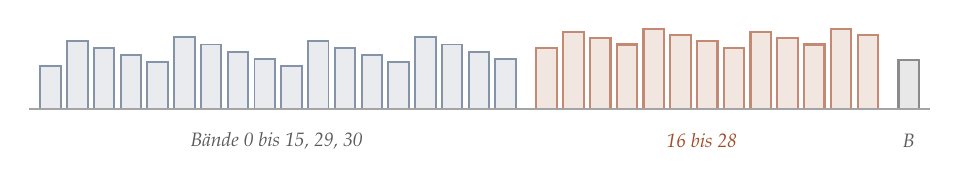
\begin{tikzpicture}[scale=1.0]
\foreach \i in {0,...,17} {
  \pgfmathsetmacro{\h}{0.55+0.045*mod(\i*7,9)}
  \draw[tief!55, line width=0.7pt, fill=tief!10] (\i*0.34-5.0,0) rectangle ++(0.26,\h);
}
\foreach \i in {0,...,12} {
  \pgfmathsetmacro{\h}{0.78+0.04*mod(\i*5,7)}
  \draw[akzent!65, line width=0.8pt, fill=akzent!14] (\i*0.34+1.3,0) rectangle ++(0.26,\h);
}
\draw[grau!70, line width=0.8pt, fill=grau!14] (5.9,0) rectangle ++(0.26,0.62);
\draw[grau!55, line width=0.6pt] (-5.15,0) -- (6.3,0);
\node[font=\scriptsize\itshape, color=grau] at (-2.0,-0.4) {Bände 0 bis 15, 29, 30};
\node[font=\scriptsize\itshape, color=akzent] at (3.4,-0.4) {16 bis 28};
\node[font=\scriptsize\itshape, color=grau] at (6.03,-0.4) {B};
\end{tikzpicture}

\vspace{1.5cm}
{\large\color{grau} Von den Grundrechenarten bis zur Darstellungstheorie}\\[6pt]
{\color{grau} Zweiunddreißig Bände, 6044 Seiten. Jeder Schritt erklärt.}\\[1.6cm]
{\small\color{grau} Herausgegeben von}\\[4pt]
{\large\color{tief} Jürgen Maier}\\[1.4cm]
{\small\color{grau} Stand der Forschung: August 2026}
\end{titlepage}
\thispagestyle{empty}
\vspace*{\fill}
\begin{flushleft}
{\small\color{grau}
\textbf{\color{tief}Mathematik von Grund auf} --- Einleitung und Gesamtverzeichnis\\[14pt]

Herausgeber und Urheber: Jürgen Maier\\[2pt]
Entstanden 2026 in Zusammenarbeit mit Claude (Anthropic); Konzeption, Vorgaben, Prüfung und Herausgeberschaft: Jürgen Maier.\\[14pt]

\textbf{Lizenz}\\[2pt]
Dieses Werk ist lizenziert unter einer Creative-Commons-Lizenz \textbf{Namensnennung -- Weitergabe unter gleichen Bedingungen 4.0 International (CC BY-SA 4.0)}. Sie dürfen das Werk vervielfältigen, verbreiten, bearbeiten und auch kommerziell nutzen, sofern Sie den Urheber nennen und Bearbeitungen unter derselben Lizenz weitergeben.\\[2pt]
Lizenztext: \texttt{https://creativecommons.org/licenses/by-sa/4.0/legalcode.de}\\[14pt]

\textbf{Quellen und Fassungen}\\[2pt]
Quelltexte, Simulationen, Fehlermeldungen und aktuelle Fassungen aller Bände:\\
\texttt{https://github.com/juergenmaier2026/mathematik-von-grund-auf}\\[2pt]
Dauerhaft archiviert bei Zenodo: \texttt{https://doi.org/10.5281/zenodo.23698547}\\[14pt]

\textbf{Zitiervorschlag}\\[2pt]
Maier, J. (2026). \textit{Mathematik von Grund auf: Einleitung und Gesamtverzeichnis}. Fassung 1.1.0. \texttt{https://doi.org/10.5281/zenodo.23698547}\\[14pt]

Satz: \LaTeX{} mit Palatino. Fassung 1.1.0, Oktober 2026.
}
\end{flushleft}
\vspace*{1.5cm}

\tableofcontents
\mainmatter

\chapter*{Einleitung zum Gesamtwerk}
\addcontentsline{toc}{chapter}{Einleitung zum Gesamtwerk}

\begin{merksatz}
\boxtitel{Das Ziel}
Dieses Werk verfolgt ein einziges Ziel: einem erwachsenen Menschen, der die Mathematik verstehen will, den Weg von null bis zur Einführungsvorlesung zu ebnen --- ohne Lücken, ohne Sprünge und ohne die Formel, die alles verdirbt: \enquote{wie man leicht sieht}.

\begin{center}
\begin{minipage}{0.9\textwidth}
\textbf{Nichts ist selbstverständlich. Nichts ist trivial. Jeder Schritt wird erklärt.}
\end{minipage}
\end{center}

\schritt{Die Regel, ausbuchstabiert}
\begin{center}
{\small
\renewcommand{\arraystretch}{1.52}
\begin{tabular}{@{}P{2.8cm}P{5.8cm}@{}}
\toprule
\textbf{Keine Regel} & ohne Begründung. Warum minus mal minus plus ergibt, steht in Band 0 auf Seite drei.\\
\textbf{Keine Formel} & die vom Himmel fällt. Die $p$-$q$-Formel wird in vier Zeilen quadratischer Ergänzung entwickelt.\\
\textbf{Kein Beweis} & mit Lücke. \enquote{Analog} und \enquote{offensichtlich} kommen nicht vor.\\
\textbf{Keine Aufgabe} & ohne vollständigen Rechenweg --- samt Zahlenprobe am Ende.\\
\bottomrule
\end{tabular}}
\end{center}

\begin{center}
\begin{minipage}{0.88\textwidth}
\kursiv{Der Grund für diese Strenge ist nicht Pedanterie, sondern Erfahrung. \textbf{Wer eine Regel ohne Begründung lernt, hat nichts, woran er sich erinnern könnte.} Wer versteht, warum sie gilt, kann sie rekonstruieren, wenn er sie vergisst.}
\end{minipage}
\end{center}
\end{merksatz}

\section*{Wie das Werk entstanden ist}
\addcontentsline{toc}{section}{Wie das Werk entstanden ist}

\begin{merksatz}
\boxtitel{Drei Bauabschnitte}
Die Bände sind nicht in der Reihenfolge geschrieben worden, in der sie hier stehen.

\begin{center}
{\small
\renewcommand{\arraystretch}{1.55}
\begin{tabular}{@{}P{2.4cm}P{6.2cm}@{}}
\toprule
\textbf{Erster} & Ein Band über den Beweisbegriff; danach Zahlentheorie, lineare Algebra, Analysis, Stochastik, Numerik, Geometrie, Geschichte, Topologie, Vektoranalysis, Logik. Elf Bände --- und dann fehlte der wichtigste.\\
\textbf{Band 0} & Alle elf hatten stillschweigend vorausgesetzt, was in der Schule gelehrt und meist wieder vergessen wird. Dieser Band trägt daher die Nummer null: Er wurde an dieser Stelle geschrieben und gehört an den Anfang.\\
\textbf{Zweiter} & Algebra, Funktionentheorie, Maßtheorie mit Funktionalanalysis, Differentialgleichungen, Kombinatorik --- die Bände 11 bis 15. Damit war der Stoff der ersten vier Semester abgedeckt.\\
\textbf{Dritter} & Elf Bände: zehn, die die vorhandenen Gebiete anwenden --- Graphentheorie, Statistik, Biomathematik, Optimierung, Informationstheorie, Spieltheorie, maschinelles Lernen, Kausalität, Entscheidungstheorie, Ökonometrie --- und einer, der eine Grundlagenlücke schließt: die stochastischen Prozesse.\\
\textbf{Vierter} & Vier Nachtragsbände: zwei Anwendungen --- numerische Simulation (27) und dynamische Systeme (28) --- und zwei Grundlagen, die in der Lückenliste der ersten Fassung standen: algebraische Geometrie (29) und Darstellungstheorie (30).\\
\bottomrule
\end{tabular}}
\end{center}

\begin{center}
\begin{minipage}{0.88\textwidth}
\kursiv{Der dritte Abschnitt hat den Charakter des Werkes verändert, und Abschnitt 1.2 behandelt das ausführlich. \textbf{Aus einem Lehrgang wurde ein Lehrgang mit Anwendungsteil} --- und die Anwendungsbände greifen so stark ineinander, dass sie eine eigene Lesart verdienen.}
\end{minipage}
\end{center}
\end{merksatz}

\begin{merksatz}
\boxtitel{Warum ein Vorkurs nötig ist}
Die Abbruchquoten in der Mathematik und den mathematiknahen Fächern gehören zu den höchsten überhaupt; der weitaus größte Teil der Abbrüche geschieht in den ersten drei Semestern.

\begin{center}
\begin{minipage}{0.9\textwidth}
\textbf{Es fehlt selten am Verständnis für den neuen Stoff. Es fehlt an der Verfügbarkeit des alten.}
\end{minipage}
\end{center}

\begin{center}
\begin{minipage}{0.88\textwidth}
\kursiv{Wer beim Ableiten von $\frac{x^{2}-1}{x+3}$ noch über das Zusammenfassen von Brüchen nachdenken muss, hat keine Aufmerksamkeit mehr für die Quotientenregel übrig --- und schon gar nicht für den Gedanken dahinter. \textbf{Deshalb steht am Anfang dieses Werkes kein Kapitel über Mengen und Abbildungen}, wie es in Vorlesungsskripten üblich ist, sondern eines über Zahlen und das Rechnen mit ihnen.}
\end{minipage}
\end{center}
\end{merksatz}

\section*{Die drei Prinzipien}
\addcontentsline{toc}{section}{Die drei Prinzipien}

\begin{merksatz}
\boxtitel{Erstens: Herkunft statt Fertigware}
Jeder Begriff wird dort abgeholt, wo er entstanden ist.

\begin{center}
{\small
\renewcommand{\arraystretch}{1.5}
\begin{tabular}{@{}P{2.8cm}P{5.8cm}@{}}
\toprule
\textbf{Die Mengenlehre} & erscheint nicht als Fundament, sondern als das, was sie war: Cantors Werkzeug für ein technisches Problem der Fourieranalyse.\\
\textbf{Der Funktionsbegriff} & kommt nicht als Definition, sondern als Dirichlets Bruch mit Euler.\\
\textbf{Das Auswahlaxiom} & kommt mit Russells Socken und Zermelos Streit mit den französischen Analytikern.\\
\bottomrule
\end{tabular}}
\end{center}

\begin{center}
\begin{minipage}{0.88\textwidth}
\kursiv{Der Grund ist didaktisch, nicht antiquarisch. \textbf{Ein Begriff, dessen Problem man kennt, ist verständlich; ein Begriff ohne Problem ist Willkür.} Ein eigener Band --- Band 7 --- ist der Geschichte gewidmet und erzählt die Entwicklung im Zusammenhang, statt sie in Fußnoten zu verteilen.}
\end{minipage}
\end{center}
\end{merksatz}

\begin{warnung}
\boxtitelr{Zweitens: Die Fehler ernst nehmen}
In jedem Band gibt es Warnkästen. Sie enthalten keine Nebensächlichkeiten, sondern die Stellen, an denen erfahrungsgemäß etwas schiefgeht:
\[ -2^{2} \ne (-2)^{2}, \qquad (a+b)^{2} \ne a^{2}+b^{2}, \qquad \sqrt{a^{2}} = |a|, \qquad f^{-1} \ne \tfrac1f \]
\[ \frac{a}{b+c} \ne \frac ab + \frac ac, \qquad \log(a+b) \ne \log a + \log b, \qquad (fg)' \ne f'g' \]

\begin{center}
\begin{minipage}{0.88\textwidth}
\kursiv{Band 0 sammelt dreiunddreißig solcher Fehler in einem Katalog, jeweils mit falscher Fassung, richtiger Fassung und Kapitelverweis. \textbf{Fehler sind keine Zufälle. Sie folgen Mustern} --- fast alle beruhen darauf, dass man eine Operation für linear hält, die es nicht ist. Wer das Muster kennt, erkennt den Fehler wieder.}
\end{minipage}
\end{center}

\schritt{In den Anwendungsbänden ändert sich die Art der Fehler}
\begin{center}
\begin{minipage}{0.88\textwidth}
\kursiv{Dort geht es nicht mehr um Rechenfehler, sondern um Anwendungsfehler: ein Modell, das nicht passt; eine Voraussetzung, die niemand geprüft hat; ein Satz, der auf einen Fall angewandt wird, den er nicht abdeckt. \textbf{Die Warnkästen heißen dort \enquote{Der Bruchfall}} und stehen in jedem Kapitel.}
\end{minipage}
\end{center}
\end{warnung}

\begin{merksatz}
\boxtitel{Drittens: Bis an den heutigen Rand}
Jeder Band endet mit einem Kapitel \enquote{Aktueller Stand} --- was heute offen ist, woran gearbeitet wird, was sich in den letzten Jahren geändert hat.

\begin{center}
{\small
\renewcommand{\arraystretch}{1.46}
\begin{tabular}{@{}P{1.8cm}P{6.4cm}@{}}
\toprule
Band 1 & Was die Riemannsche Vermutung mit Primzahlen zu tun hat\\
Band 3 & Die Navier-Stokes-Gleichungen als Millenniumsproblem\\
Band 5 & Warum P gegen NP die Numerik betrifft\\
Band 8 & Die Poincaré-Vermutung und Perelmans Beweis\\
Band 10 & Woodins Programm zur Kontinuumshypothese\\
Band 17 & Die Replikationskrise und was aus ihr folgt\\
Band 19 & Wo lineare Optimierung an ihre Grenzen stößt\\
Band 20 & Kryptographie nach dem Quantenrechner\\
Band 21 & Warum Menschen nicht spielen, was die Theorie sagt\\
Band 22 & Warum tiefe Netze verallgemeinern, obwohl sie es nicht dürften\\
Band 23 & Warum dieselbe Tabelle mit entgegengesetzten Ursachen vereinbar ist\\
Band 24 & Warum ein Test nur zwischen zwei Schwellen etwas nützt\\
Band 25 & Warum beim fairen Spiel meist einer fast durchgehend führt\\
Band 26 & Warum zwei unabhängige Zeitreihen meist signifikant zusammenhängen\\
Band 27 & Warum ein Simulationsergebnis ohne Fehlerbalken keines ist\\
Band 28 & Warum man das Wetter nicht über zwei Wochen hinaus vorhersagen kann\\
Band 29 & Warum Gröbner-Basen entscheiden, welche Parameter ein Modell preisgibt\\
Band 30 & Warum die McKay-Vermutung nach fünfzig Jahren bewiesen ist\\
\bottomrule
\end{tabular}}
\end{center}

\begin{center}
\begin{minipage}{0.9\textwidth}
\textbf{Der Stand ist überall der August 2026.}
\end{minipage}
\end{center}

\begin{center}
\begin{minipage}{0.88\textwidth}
\kursiv{Nicht, weil man das für die Prüfung braucht, sondern weil Mathematik sonst wie ein abgeschlossenes Gebäude wirkt. \textbf{Sie ist es nicht.}}
\end{minipage}
\end{center}
\end{merksatz}

\section*{Was das Werk nicht ist}
\addcontentsline{toc}{section}{Was das Werk nicht ist}

\begin{warnung}
\boxtitelr{Vier ehrliche Einschränkungen}
\begin{center}
{\small
\renewcommand{\arraystretch}{1.55}
\begin{tabular}{@{}P{2.4cm}P{6.2cm}@{}}
\toprule
\textbf{Erstens} & Es ist kein Ersatz für das Üben. Wer die durchgerechneten Aufgaben nur liest, statt sie mitzurechnen, wird beim ersten eigenen Problem stehen. Papier und Stift sind Teil der Ausrüstung.\\
\textbf{Zweitens} & Es ist keine Vollständigkeitserklärung. Die zweite Werkhälfte und die Nachtragsbände haben viele Lücken geschlossen --- diskrete Mathematik, Statistik, Optimierung, algebraische Geometrie, Darstellungstheorie, numerische Simulation ---, andere bleiben offen: Lie-Gruppen und -Algebren systematisch, partielle Differentialgleichungen in der Tiefe, algebraische Zahlentheorie, Differentialgeometrie.\\
\textbf{Drittens} & Es ersetzt keine Vorlesung. Es soll sie verständlich machen.\\
\textbf{Viertens} & Es ist nicht neutral. Wo es mehrere Zugänge gibt, ist einer gewählt und begründet worden --- und die Begründung steht dabei.\\
\bottomrule
\end{tabular}}
\end{center}

\begin{center}
\begin{minipage}{0.88\textwidth}
\kursiv{Zur zweiten Einschränkung eine Bemerkung: \textbf{Die ursprüngliche Fassung dieser Liste nannte Algebra, Funktionentheorie, Maßtheorie, Differentialgleichungen und Kombinatorik als fehlend.} Sie sind inzwischen die Bände 11 bis 15; die zweite Fassung nannte algebraische Geometrie, Darstellungstheorie und numerische Simulation --- sie sind die Bände 29, 30 und 27. Eine Lückenliste ist ein Arbeitsplan, kein Bekenntnis.}
\end{minipage}
\end{center}
\end{warnung}

\begin{merksatz}
\boxtitel{Und ein Wort zur Zählung}
\begin{center}
{\small
\renewcommand{\arraystretch}{1.5}
\begin{tabular}{@{}P{2.4cm}P{2.4cm}P{2.6cm}@{}}
\toprule
\textbf{Bände} & \textbf{Anzahl} & \textbf{Seiten}\\
\midrule
$0$ bis $15$, $29$, $30$ und $B$ & $19$ & $3348$\\
$16$ bis $28$ & $13$ & $2696$\\
\midrule
\textbf{Zusammen} & $\mathbf{32}$ & $\mathbf{6044}$\\
\bottomrule
\end{tabular}}
\end{center}

\begin{center}
\begin{minipage}{0.88\textwidth}
\kursiv{Der vorliegende Rahmenband ist nicht mitgezählt. \textbf{Der Begleitband \enquote{Die Architektur der Gewissheit} trägt keine Nummer}, weil er als erster entstand und sich mit Band 10 teilweise überschneidet. Wer nur einen von beiden liest, nehme Band 10 für die Technik und den Begleitband für die Einordnung.}
\end{minipage}
\end{center}
\end{merksatz}

\chapter{Die zweiunddreißig Bände}

\section{Übersicht}

\begin{center}
{\small
\renewcommand{\arraystretch}{1.42}
\begin{longtable}{@{}P{1.4cm}P{4.2cm}P{4.2cm}P{1.3cm}@{}}
\toprule
\textbf{Band} & \textbf{Titel} & \textbf{Gebiet} & \textbf{Seiten}\\
\midrule
\endhead
$0$ & Die Kunst des Rechnens & Vorkurs Schulmathematik & $154$\\
$1$ & Die Königin der Mathematik & Zahlentheorie & $181$\\
$2$ & Die Kunst der linearen Struktur & Lineare Algebra & $167$\\
$3$ & Die Kunst des Grenzübergangs & Analysis & $173$\\
$4$ & Die Vermessung des Zufalls & Wahrscheinlichkeitstheorie & $164$\\
$5$ & Die Kunst der Näherung & Numerische Mathematik & $224$\\
$6$ & Die Vermessung des Raumes & Geometrie & $184$\\
$7$ & Die Wege des Denkens & Geschichte der Mathematik & $188$\\
$8$ & Die Kunst der Verformung & Topologie & $178$\\
$9$ & Die Sprache der Felder & Vektor- und Tensoranalysis & $130$\\
$10$ & Die Ordnung des Unendlichen & Logik und Mengenlehre & $124$\\
$11$ & Die Gestalt der Symmetrie & Algebra & $150$\\
$12$ & Die Vollendung der Analysis & Funktionentheorie & $176$\\
$13$ & Das Maß und der Raum & Maßtheorie, Funktionalanalysis & $175$\\
$14$ & Die Gesetze der Veränderung & Differentialgleichungen & $214$\\
$15$ & Die Kunst des Zählens & Kombinatorik & $200$\\
\midrule
$16$ & Punkte und Linien & Graphentheorie & $270$\\
$17$ & Was die Zahlen hergeben & Statistik & $282$\\
$18$ & Wachsen und Vergehen & Biomathematik & $262$\\
$19$ & Das Beste finden & Optimierung & $252$\\
$20$ & Was Nachrichten wiegen & Information, Kryptographie & $242$\\
$21$ & Wenn andere mitrechnen & Spieltheorie & $236$\\
$22$ & Was sich verallgemeinern lässt & Maschinelles Lernen & $204$\\
$23$ & Woran es liegt & Kausale Schlüsse & $158$\\
$24$ & Was zu tun ist & Entscheidungen unter Unsicherheit & $140$\\
$25$ & Wenn der Zufall weitergeht & Stochastische Prozesse & $158$\\
$26$ & Wenn die Daten sich selbst bestimmen & Ökonometrie & $156$\\
$27$ & Was der Rechner vom Zufall weiß & Numerische Simulation & $170$\\
$28$ & Wo die Vorhersage endet & Dynamische Systeme und Chaos & $166$\\
\midrule
$29$ & Die Form der Lösungen & Algebraische Geometrie & $188$\\
$30$ & Was die Symmetrie verrät & Darstellungstheorie & $196$\\
\midrule
$B$ & Die Architektur der Gewissheit & Beweistheorie (Begleitband) & $182$\\
\midrule
\textbf{Gesamt} & & & $\mathbf{6044}$\\
\bottomrule
\end{longtable}}
\end{center}

\section{Die beiden Hälften des Werkes}

\begin{merksatz}
\boxtitel{Ein Unterschied, der sich im Aufbau zeigt}
\begin{center}
{\small
\renewcommand{\arraystretch}{1.55}
\begin{tabular}{@{}P{2.2cm}P{3.0cm}P{3.2cm}@{}}
\toprule
& \textbf{Bände 0 bis 15, 29, 30} & \textbf{Bände 16 bis 28}\\
\midrule
Aufbau & systematisch nach Gebiet & nach Anwendung\\
Reihenfolge & aufeinander aufbauend & je Band eigenständig\\
Beispiele & wechselnd & \textcolor{akzent}{ein durchgehender Leitfall}\\
Ziel & den Stoff verfügbar machen & ihn benutzen können\\
Bezüge & innerhalb des Gebiets & quer durch die erste Hälfte\\
\bottomrule
\end{tabular}}
\end{center}

\begin{center}
\begin{minipage}{0.9\textwidth}
\textbf{Die erste Hälfte fragt: Was ist das und warum stimmt es? Die zweite: Wozu ist es gut und wann versagt es?}
\end{minipage}
\end{center}
\end{merksatz}

\begin{merksatz}
\boxtitel{Der Leitfall}
Jeder der zwölf Anwendungsbände hat ein durchgehendes Beispiel, das vom ersten bis zum letzten Kapitel mitläuft.

\begin{center}
{\small
\renewcommand{\arraystretch}{1.5}
\begin{tabular}{@{}P{1.2cm}P{7.0cm}@{}}
\toprule
$16$ & Das Kontaktnetz einer Station --- von der Gradfolge bis zur Ausbreitung.\\
$17$ & Die MOBIL-Studie zum Hüftgelenksersatz --- von der Beschreibung bis zur Metaanalyse.\\
$18$ & Neustadt und sein Klinikum --- Epidemie, Pharmakokinetik, Tumorwachstum, Resistenz.\\
$19$ & Zwei Eingriffsarten unter knapper OP-Zeit --- von der Ecke bis zum Schattenpreis.\\
$20$ & Die Digitalisierung des Klinikums --- Diagnoseschlüssel, Funkstrecke, Arztbrief.\\
$21$ & Klinikum und Marienhospital --- Standort, Reserveantibiotikum, Dienstplan.\\
$22$ & Die Sepsis-Frühwarnung --- vom Laktatwert bis zum tiefen Netz.\\
$23$ & Die frühe Antibiotikagabe --- eine Tabelle mit falschem Vorzeichen.\\
$24$ & Frau B.\ mit Vorhofflimmern --- Schlaganfall gegen Blutung.\\
$25$ & Die Intensivstation als Prozess --- Ankünfte, Belegung, Wartezeiten.\\
$26$ & Zuzahlung und Arztbesuch --- Experiment, Praxisgebühr, Panel.\\
$27$ & Dieselbe Intensivstation im Rechner --- von der Zufallszahl bis zur Unsicherheit des Ergebnisses.\\
$28$ & Die Herzzelle --- Ruhe, Takt, Flimmern, und wo die Vorhersage endet.\\
\bottomrule
\end{tabular}}
\end{center}

\begin{center}
\begin{minipage}{0.88\textwidth}
\kursiv{Die Wahl des Gegenstands ist nicht zufällig: \textbf{Ein Krankenhaus ist ein Ort, an dem Zahlen Folgen haben} --- und an dem sich gut zeigen lässt, warum eine falsche Modellannahme nicht nur ein Rechenfehler ist. Wer aus einem anderen Fach kommt, kann die Leitfälle ohne Vorkenntnisse lesen; sie sind durchgehend erklärt.}
\end{minipage}
\end{center}
\end{merksatz}

\begin{merksatz}
\boxtitel{Wie die Anwendungsbände zusammenhängen}
\begin{center}
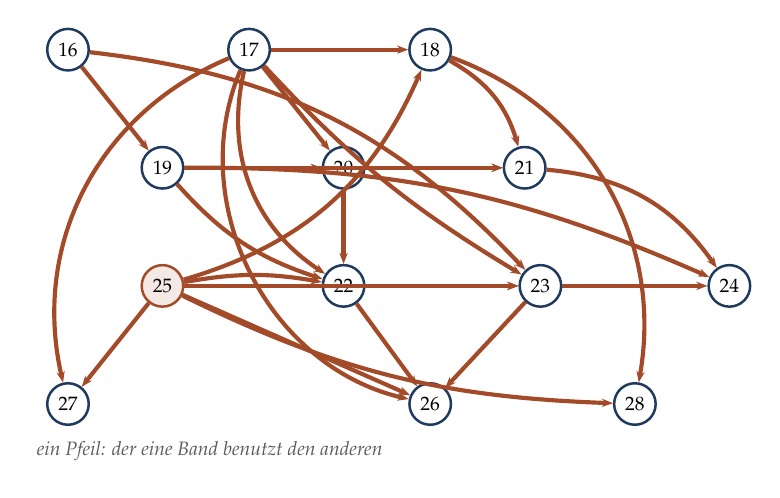
\begin{tikzpicture}[scale=1.0]
\node[knotenb] (b16) at (-3.4,1.5) {16};
\node[knotenb] (b17) at (-1.1,1.5) {17};
\node[knotenb] (b18) at (1.2,1.5) {18};
\node[knotenb] (b19) at (-2.2,0) {19};
\node[knotenb] (b20) at (0.1,0) {20};
\node[knotenb] (b21) at (2.4,0) {21};
\node[knotenb] (b22) at (0.1,-1.5) {22};
\node[knotenb] (b23) at (2.6,-1.5) {23};
\node[knotenb] (b24) at (5.0,-1.5) {24};
\node[knotenr] (b25) at (-2.2,-1.5) {25};
\node[knotenb] (b26) at (1.2,-3.0) {26};
\node[knotenb] (b27) at (-3.4,-3.0) {27};
\node[knotenb] (b28) at (3.8,-3.0) {28};
\draw[kanted, -{Stealth[length=4pt]}] (b17)--(b18);
\draw[kanted, -{Stealth[length=4pt]}] (b17)--(b20);
\draw[kanted, -{Stealth[length=4pt]}] (b16)--(b19);
\draw[kanted, -{Stealth[length=4pt]}] (b19)--(b20);
\draw[kanted, -{Stealth[length=4pt]}] (b19)--(b21);
\draw[kanted, -{Stealth[length=4pt]}] (b20)--(b21);
\draw[kanted, -{Stealth[length=4pt]}] (b18) to[bend left=22] (b21);
\draw[kanted, -{Stealth[length=4pt]}] (b17) to[bend right=35] (b22);
\draw[kanted, -{Stealth[length=4pt]}] (b19) to[bend right=15] (b22);
\draw[kanted, -{Stealth[length=4pt]}] (b20)--(b22);
\draw[kanted, -{Stealth[length=4pt]}] (b22)--(b23);
\draw[kanted, -{Stealth[length=4pt]}] (b23)--(b24);
\draw[kanted, -{Stealth[length=4pt]}] (b19) to[bend left=12] (b24);
\draw[kanted, -{Stealth[length=4pt]}] (b21) to[bend left=25] (b24);
\draw[kanted, -{Stealth[length=4pt]}] (b25) to[bend left=10] (b22);
\draw[kanted, -{Stealth[length=4pt]}] (b25) to[bend right=25] (b18);
\draw[kanted, -{Stealth[length=4pt]}] (b25)--(b23);
\draw[kanted, -{Stealth[length=4pt]}] (b17) to[bend right=50] (b26);
\draw[kanted, -{Stealth[length=4pt]}] (b22)--(b26);
\draw[kanted, -{Stealth[length=4pt]}] (b23)--(b26);
\draw[kanted, -{Stealth[length=4pt]}] (b25)--(b26);
\draw[kanted, -{Stealth[length=4pt]}] (b25)--(b27);
\draw[kanted, -{Stealth[length=4pt]}] (b17) to[bend right=40] (b27);
\draw[kanted, -{Stealth[length=4pt]}] (b25) to[bend right=12] (b28);
\draw[kanted, -{Stealth[length=4pt]}] (b18) to[bend left=40] (b28);
\draw[kanted, -{Stealth[length=4pt]}] (b16) to[bend left=20] (b23);
\draw[kanted, -{Stealth[length=4pt]}] (b17) to[bend right=8] (b23);

\node[font=\scriptsize\itshape, color=grau] at (-1.6,-3.6) {ein Pfeil: der eine Band benutzt den anderen};
\end{tikzpicture}
\end{center}

\begin{center}
{\small
\renewcommand{\arraystretch}{1.5}
\begin{tabular}{@{}P{2.0cm}P{6.4cm}@{}}
\toprule
$17 \to 18$ & Schätzen und Testen für Modellanpassung und Studienauswertung.\\
$17 \to 20$ & Die relative Entropie erscheint dort als Werkzeug der Modellwahl.\\
$16 \to 19$ & Flüsse und Zuordnungen als ganzzahlige lineare Programme.\\
$19 \to 20$ & Dualität und Konvexität hinter der Kanalkapazität.\\
$19 \to 21$ & Der Minimax-Satz ist der Dualitätssatz.\\
$20 \to 21$ & Robuste Optimierung als Spiel gegen die Natur.\\
$18 \to 21$ & Resistenz als evolutionäres Spiel --- die Rechnung, die Band 18 offenließ.\\
$17,\,19,\,20 \to 22$ & Schätzen, Minimieren und die kürzeste Beschreibung treffen sich im Lernen.\\
$16,\,17,\,22 \to 23$ & Graphen tragen die Annahmen, das Lernen die Schätzer.\\
$19,\,21,\,23 \to 24$ & Wirkung, Kosten und Gegenspieler treffen sich in der Wahl.\\
$25 \to 18,\,22,\,23$ & Der einzige Band der zweiten Hälfte, der Grundlagen nachliefert statt anzuwenden.\\
$17,\,22,\,23,$ $25 \to 26$ & Der Band, der die meisten Vorgänger zugleich braucht --- und sie unter erschwerten Bedingungen zusammenführt.\\
\bottomrule
\end{tabular}}
\end{center}

\begin{center}
\begin{minipage}{0.88\textwidth}
\kursiv{\textbf{Die letzte Zeile ist die engste Verbindung des ganzen Werkes.} Band 18 behandelt in Kapitel~14 die adaptive Tumortherapie und bemerkt, das Wettrüsten zwischen Therapie und Resistenz sei im Kern ein Spiel --- ohne die Rechnung zu führen. Band 21 führt sie in Kapitel~10 mit denselben Zahlen aus: Startanteil $10^{-6}$, Eignungsdifferenzen $+0{,}04$ und $-0{,}01$ je Tag, Ergebnis $T_{\text{aus}} \ge 4\,T_{\text{an}}$.}
\end{minipage}
\end{center}
\end{merksatz}

\section{Was in welchem Band steht}

\begin{merksatz}
\boxtitel{Band 0 --- Die Kunst des Rechnens}
Die gesamte Schulmathematik, jede Regel begründet. Zahlbereiche und der Irrationalitätsbeweis für $\sqrt2$; Bruchrechnung mit drei Begründungen für den Kehrwert; Potenzen, Wurzeln, Logarithmen als eine Familie; Terme, Gleichungen, Ungleichungen mit Beträgen; der Funktionsbegriff und die acht Grundtypen; Geometrie und Trigonometrie; Folgen, Ableitung, Integral; Beweisen lernen.

\kursiv{Besonderheit: ein Fehlerkatalog mit dreiunddreißig Einträgen und ein Schlusskapitel über die Lernforschung.}
\end{merksatz}

\begin{merksatz}
\boxtitel{Band 1 --- Die Königin der Mathematik}
Zahlentheorie von der Teilbarkeit bis zu elliptischen Kurven. Euklidischer Algorithmus, Fundamentalsatz der Arithmetik, modulares Rechnen, chinesischer Restsatz, die Sätze von Fermat, Euler und Wilson, quadratische Reziprozität, Primzahlverteilung, diophantische Gleichungen, Kettenbrüche, RSA und Primzahltests.

\kursiv{Der Titel stammt von Gauß, der die Zahlentheorie die Königin der Mathematik nannte.}
\end{merksatz}

\begin{merksatz}
\boxtitel{Band 2 --- Die Kunst der linearen Struktur}
Lineare Algebra vom Gleichungssystem bis zur Singulärwertzerlegung. Der Aufbau geht bewusst vom Konkreten zum Abstrakten: erst Gauß-Algorithmus und Matrizen, dann der Vektorraumbegriff, dann lineare Abbildungen, Determinante, Eigenwerte, Jordanform, Skalarprodukte, Spektralsatz.

\kursiv{Die Singulärwertzerlegung ist der Grund, warum dieser Band für alle Anwendungsgebiete zentral ist --- von der Bildkompression bis zum maschinellen Lernen.}
\end{merksatz}

\begin{merksatz}
\boxtitel{Band 3 --- Die Kunst des Grenzübergangs}
Analysis in der strengen Fassung. Konstruktion der reellen Zahlen, Folgen und Reihen, Stetigkeit, die elementaren Funktionen, Differentialrechnung mit Mittelwertsätzen und Taylor, Riemann-Integral und Hauptsatz, gleichmäßige Konvergenz, Differentialrechnung im $\R^{n}$.

\kursiv{Der Unterschied zu Band 0: Dort wird gerechnet, hier wird bewiesen. Die $\varepsilon$-$\delta$-Definition ist der Angelpunkt.}
\end{merksatz}

\begin{merksatz}
\boxtitel{Band 4 --- Die Vermessung des Zufalls}
Wahrscheinlichkeitstheorie von null an, einschließlich der Schulstochastik. Kombinatorik, bedingte Wahrscheinlichkeit und das Ziegenproblem, Zufallsvariablen, die diskreten und stetigen Verteilungen, Erwartungswert und Varianz, die Gesetze der großen Zahlen, der zentrale Grenzwertsatz, Markow-Ketten, Martingale, Schätzen und Testen.

\kursiv{Wer die Schulstochastik wiederholen will, findet sie hier --- deshalb fehlt sie in Band 0.}
\end{merksatz}

\begin{merksatz}
\boxtitel{Band 5 --- Die Kunst der Näherung}
Numerische Mathematik. Gleitkommazahlen und ihre Tücken, Kondition und Stabilität, LR- und QR-Zerlegung, iterative Verfahren, Eigenwertberechnung, Nullstellenverfahren, Interpolation und Splines, Quadratur, Anfangs- und Randwertprobleme, Optimierung, Monte-Carlo.

\kursiv{Der Band beginnt mit einer Warnung: $0{,}1+0{,}2 \ne 0{,}3$ im Rechner --- und erklärt, warum das so ist und was daraus folgt.}
\end{merksatz}

\begin{merksatz}
\boxtitel{Band 6 --- Die Vermessung des Raumes}
Geometrie in allen ihren Gestalten. Euklid und die Axiome, Dreieck und Kegelschnitte, analytische Geometrie, Isometrien und Symmetriegruppen, projektive Geometrie, das Parallelenproblem, hyperbolische und sphärische Geometrie, Kurven- und Flächentheorie bis Gauß-Bonnet, diskrete Geometrie und Packungen.

\kursiv{Das Parallelenproblem ist die Achse des Bandes --- zweitausend Jahre Bemühen um einen Beweis, der nicht zu führen war.}
\end{merksatz}

\begin{merksatz}
\boxtitel{Band 7 --- Die Wege des Denkens}
Die Geschichte der Mathematik im Zusammenhang. Von den Zahlzeichen über China, Indien und Mesoamerika, das griechische Wunder, die islamische Welt, Renaissance, die Revolution des 17.\ Jahrhunderts, die Rigorisierung des 19., die Grundlagenkrise des 20.\ --- bis zu Vertreibung, Krieg und der Mathematik von heute.

\kursiv{Der Band ist ohne Vorkenntnisse lesbar und eignet sich als Einstieg für alle, die wissen wollen, worum es überhaupt geht.}
\end{merksatz}

\begin{merksatz}
\boxtitel{Band 8 --- Die Kunst der Verformung}
Topologie vom metrischen Raum bis zur Homologie. Offene Mengen, Stetigkeit ohne $\varepsilon$, Kompaktheit und Zusammenhang, Trennungsaxiome, Quotientenräume, Fundamentalgruppe und Überlagerungen, Homologie, Fixpunktsätze, Mannigfaltigkeiten und die Klassifikation der Flächen.

\kursiv{Der Fixpunktsatz von Brouwer taucht in vier weiteren Bänden wieder auf --- zuletzt in Band 21 als Grundlage des Existenzsatzes für Gleichgewichte.}
\end{merksatz}

\begin{merksatz}
\boxtitel{Band 9 --- Die Sprache der Felder}
Vektor- und Tensoranalysis. Skalar- und Vektorfelder, Gradient, Divergenz, Rotation, Kurven- und Flächenintegrale, die Sätze von Green, Gauß und Stokes, krummlinige Koordinaten, Tensoren, Differentialformen und der allgemeine Satz von Stokes.

\kursiv{Die Pointe des Bandes: Die drei Integralsätze sind ein einziger Satz, in drei Gestalten.}
\end{merksatz}

\begin{merksatz}
\boxtitel{Band 10 --- Die Ordnung des Unendlichen}
Logik und Mengenlehre. Aussagen- und Prädikatenlogik, Beweiskalküle, Vollständigkeits- und Kompaktheitssatz, ZFC mit allen Axiomen, Ordinal- und Kardinalzahlen, Auswahlaxiom und seine Äquivalente, Berechenbarkeit, die Unvollständigkeitssätze, Unabhängigkeit und die Kontinuumshypothese.

\kursiv{Überschneidet sich mit dem Begleitband B: Band 10 liefert die Technik, der Begleitband die Einordnung.}
\end{merksatz}

\begin{merksatz}
\boxtitel{Band 11 --- Die Gestalt der Symmetrie}
Algebra von der Gruppe bis zur Galoistheorie. Gruppen, Untergruppen, Satz von Lagrange, Normalteiler und Faktorgruppen, Gruppenoperationen und Sylowsätze, Ringe und Ideale, Polynomringe, Körpererweiterungen, Konstruierbarkeit mit Zirkel und Lineal, endliche Körper, die Galoiskorrespondenz und die Unlösbarkeit der Quintik.

\kursiv{Die drei klassischen Unmöglichkeiten --- Würfelverdopplung, Winkeldreiteilung, Quadratur des Kreises --- werden vollständig bewiesen.}
\end{merksatz}

\begin{merksatz}
\boxtitel{Band 12 --- Die Vollendung der Analysis}
Funktionentheorie. Komplexe Zahlen, Holomorphie und die Cauchy-Riemann-Gleichungen, der Cauchysche Integralsatz, Potenz- und Laurentreihen, der Residuensatz mit Anwendungen auf reelle Integrale, konforme Abbildungen, der Riemannsche Abbildungssatz, analytische Fortsetzung, Gamma- und Zetafunktion.

\kursiv{Der Band heißt so, weil in ihm zusammenläuft, was in den Bänden 2, 3 und 9 getrennt entwickelt wurde.}
\end{merksatz}

\begin{merksatz}
\boxtitel{Band 13 --- Das Maß und der Raum}
Maßtheorie und Funktionalanalysis. Die drei Defekte des Riemann-Integrals, $\sigma$-Algebren und Maße, das Lebesgue-Maß und die Menge von Vitali, messbare Funktionen, die Konvergenzsätze, Fubini, die $L^{p}$-Räume, Banach- und Hilberträume, Hahn-Banach und die drei Prinzipien, kompakte Operatoren, der Spektralsatz.

\kursiv{Das Schlusskapitel zeigt, warum die Quantenmechanik ohne diesen Band nicht formulierbar wäre.}
\end{merksatz}

\begin{merksatz}
\boxtitel{Band 14 --- Die Gesetze der Veränderung}
Differentialgleichungen. Richtungsfeld und elementare Lösungsverfahren, Existenz und Eindeutigkeit nach Picard-Lindelöf, lineare Systeme und das Matrixexponential, Schwingungen und Resonanz, Sturm-Liouville, Phasenporträt und Stabilität, Bifurkationen und Chaos, die drei klassischen partiellen Gleichungen, schwache Lösungen und finite Elemente.

\kursiv{Der Band ist die Brücke zwischen Analysis und Anwendung --- und die unmittelbare Grundlage von Band 18.}
\end{merksatz}

\begin{merksatz}
\boxtitel{Band 15 --- Die Kunst des Zählens}
Kombinatorik. Die Grundregeln und das Schubfachprinzip, die vier Grundaufgaben, das Pascalsche Dreieck, Inklusion und Exklusion, erzeugende Funktionen, Catalan- und Stirlingzahlen, Partitionen, Burnside und Pólya, Graphen, Ramseytheorie, die probabilistische Methode, extremale Mengenlehre.

\kursiv{Der Graphenteil ist hier ein Kapitel; Band 16 macht ein eigenes Buch daraus.}
\end{merksatz}

\begin{merksatz}
\boxtitel{Band 16 --- Punkte und Linien}
Graphentheorie als eigenständiger Band. Vom Graphbegriff über Wege und Zusammenhang, Bäume und Spannbäume, Eulerkreise und Hamiltonkreise, Planarität und der Vierfarbensatz, Färbungen, Matchings und der Satz von Hall, Flüsse und Schnitte, Zufallsgraphen, Netzwerke und Zentralitätsmaße.

\kursiv{Leitfall ist das Kontaktnetz einer Station --- vom Handschlaglemma bis zur Ausbreitungsschwelle. Der erste Band der zweiten Werkhälfte.}
\end{merksatz}

\begin{merksatz}
\boxtitel{Band 17 --- Was die Zahlen hergeben}
Statistik von der Beschreibung bis zur Metaanalyse. Lage- und Streumaße, Schätzen, Konfidenzintervalle, Tests und ihre Fehler, Fallzahlplanung, lineare und logistische Regression, Überlebenszeitanalyse, Bayessche Verfahren, Studiendesign, multiples Testen, Metaanalyse.

\kursiv{Leitfall ist die MOBIL-Studie zum Hüftgelenksersatz. Der Band nimmt die Replikationskrise zum Anlass, jede Methode auch daran zu messen, wie leicht sie sich missbrauchen lässt.}
\end{merksatz}

\begin{merksatz}
\boxtitel{Band 18 --- Wachsen und Vergehen}
Biomathematik. Exponentielles und logistisches Wachstum, Chaos in der Rekursion, Lotka-Volterra und Wettbewerbsmodelle, Stabilität, SIR-Modelle und Impfschwellen, Ausbreitung auf Netzwerken, Pharmakokinetik, Enzymkinetik, erregbare Systeme, Tumorwachstum nach Gompertz, Resistenz und adaptive Therapie.

\kursiv{Leitfall ist Neustadt mit seinen $100\,000$ Einwohnern und seinem Klinikum. Der Band benutzt die Bände 14 und 17 unmittelbar.}
\end{merksatz}

\begin{merksatz}
\boxtitel{Band 19 --- Das Beste finden}
Optimierung. Lineare Programme und das Simplexverfahren, Dualität und Schattenpreise, totale Unimodularität, Konvexität, Lagrange und Karush-Kuhn-Tucker, Gradienten- und Newtonverfahren, ganzzahlige Optimierung, Verzweigen und Beschränken, Komplexität, Optimierung unter Unsicherheit, mehrere Ziele.

\kursiv{Leitfall ist die Planung zweier Eingriffsarten unter knapper OP-Zeit. Kapitel~4 enthält die Bemerkung, die Band 21 aufgreift: dass von Neumann in Dantzigs Problem sein eigenes wiedererkannte.}
\end{merksatz}

\begin{merksatz}
\boxtitel{Band 20 --- Was Nachrichten wiegen}
Informationstheorie und Kryptographie in einem Band. Informationsgehalt und Entropie, Quellencodierung und Huffman, Transinformation und Kanalkapazität, das Kanalcodierungstheorem, fehlerkorrigierende Codes, Kolmogorow-Komplexität, Information in der Statistik, perfekte Sicherheit, Blockchiffren, Hashfunktionen, Diffie-Hellman, RSA, elliptische Kurven.

\kursiv{Die Klammer des Bandes: Dieselbe Größe misst, was ankommen soll, und was nicht ankommen darf.}
\end{merksatz}

\begin{merksatz}
\boxtitel{Band 21 --- Wenn andere mitrechnen}
Spieltheorie. Nullsummenspiele und der Minimax-Satz, Spiele als lineare Programme, das Nash-Gleichgewicht, die klassischen Dilemmata, Existenz und Berechenbarkeit, extensive Form und Glaubwürdigkeit, wiederholte Spiele, evolutionär stabile Strategien, Replikatordynamik, Kollektivgüter, Abstimmungsverfahren, Auktionen, Verhandlung und Koalitionen.

\kursiv{Leitfall sind Klinikum und Marienhospital in Neustadt. Der Band schließt die Rechnung ab, die Band 18 offenließ.}
\end{merksatz}

\begin{merksatz}
\boxtitel{Band 22 --- Was sich verallgemeinern lässt}
Maschinelles Lernen. Die Lernaufgabe und die Bayes-Regel, Verzerrung und Varianz, Kreuzvalidierung und Datenlecks, Regularisierung mit Kamm und Lasso, logistische Regression und Perzeptron, Stützvektoren und Kerne, PAC-Lernen und VC-Dimension, Verallgemeinerungsschranken, Bäume und Wälder, nächste Nachbarn, neuronale Netze, Gruppenbildung, Hauptkomponenten, tiefe Netze und der doppelte Abstieg.

\kursiv{Leitfall ist die Sepsis-Frühwarnung --- und als Maßstab die Nachprüfung eines kommerziellen Warnsystems von 2021, die seinen Fehlschlag offenlegte. Der Band benutzt die Bände 17, 19 und 20 durchgehend.}
\end{merksatz}

\begin{merksatz}
\boxtitel{Band 23 --- Woran es liegt}
Kausale Schlüsse. Zusammenhang und Ursache, potentielle Ergebnisse, Randomisierung, kausale Graphen und d-Trennung, zulässige Anpassungsmengen, Hintertür- und Vordertürformel, Behandlungsneigung, Gewichtung und doppelte Absicherung, Instrumentvariablen, Regressionssprung und doppelte Differenz, Zielstudienemulation, g-Formel, Mediation, heterogene Effekte.

\kursiv{Leitfall ist die frühe Antibiotikagabe bei Sepsis --- eine Tabelle, die das Gegenteil dessen zeigt, was die Leitlinien sagen. Der Band benutzt die Bände 16, 17 und 22 und schließt die zweite Werkhälfte ab.}
\end{merksatz}

\begin{merksatz}
\boxtitel{Band 24 --- Was zu tun ist}
Entscheidungen unter Unsicherheit. Erwartungsnutzen und Behandlungsschwelle, Nutzenaxiome und Risikoscheu, Wert der Information, Test- und Behandlungsschwellen, Entscheidungsbäume und Empfindlichkeitsanalyse, Markow-Modelle und QALY, Rückwärtsrechnung, Markow-Entscheidungsprozesse, Erkunden gegen Ausnutzen, Kosten-Wirksamkeit, Ambiguität, tatsächliches Entscheidungsverhalten, Gruppenentscheidungen, Priorisierung.

\kursiv{Leitfall ist Frau B.\ mit Vorhofflimmern: Schlaganfall gegen Blutung. Der Band benutzt die Bände 19, 21 und 23 und schließt an die Frage an, die der kausale Schluss offenlässt.}
\end{merksatz}

\begin{merksatz}
\boxtitel{Band 25 --- Wenn der Zufall weitergeht}
Stochastische Prozesse. Irrfahrten und das Arkussinus-Gesetz, Markow-Ketten und stationäre Verteilungen, Poisson-Prozesse, Warteschlangen, Verzweigungsprozesse, bedingte Erwartung und Filtration, Martingale und optionales Stoppen, Konvergenzsätze, Brownsche Bewegung, Itō-Integral und Itō-Formel, Optionsbewertung, Prozesse in Klinik und Natur.

\kursiv{Der einzige Band der zweiten Werkhälfte, der eine Grundlagenlücke schließt: Sechs frühere Bände hatten den Prozessbegriff gebraucht und jeweils nur so weit entwickelt, wie es gerade nötig war.}
\end{merksatz}

\begin{merksatz}
\boxtitel{Band 26 --- Wenn die Daten sich selbst bestimmen}
Ökonometrie. Endogenität, Identifikation und Abzählbedingung, Instrumentvariablen und schwache Instrumente, verallgemeinerte Momentenmethode, Logit, Probit und Tobit, Auswahlmodelle, feste Effekte, dynamische Panels, doppelte Differenz und gestaffelte Einführung, Stationarität, Scheinregression und Einheitswurzeln, Kointegration und Fehlerkorrektur, Vektorautoregression, Lucas-Kritik, Vorhersage gegen Politik.

\kursiv{Leitfall ist die Wirkung von Zuzahlungen auf Arztbesuche, gemessen am Krankenversicherungsexperiment und an der Praxisgebühr. Der Band verbindet die Bände 17, 22, 23 und 25 --- kausale Fragen, Beobachtungsdaten, rückgekoppelte Systeme und nichtstationäre Zeitreihen zugleich.}
\end{merksatz}

\begin{merksatz}
\boxtitel{Band 27 --- Was der Rechner vom Zufall weiß}
Numerische Simulation. Pseudozufallszahlen und ihre Prüfung, Inversion, Verwerfung und Box--Muller, Monte-Carlo-Integration und der Fluch der Dimension, Standardfehler bei Abhängigkeit, Varianzreduktion (antithetisch, Kontrollvariable, Schichtung), Wichtigkeitsstichprobe, Metropolis und Gibbs, Konvergenzdiagnostik, Hamilton-Monte-Carlo, Pfade stochastischer Differentialgleichungen, ereignisgesteuerte Simulation, seltene Ereignisse, Teilchenfilter, Reproduzierbarkeit, Unsicherheit des Ergebnisses.

\kursiv{Leitfall ist die Intensivstation aus Band 25, diesmal als Programm: Jede Tabelle des Bandes entsteht aus einem Skript, das beiliegt. Der Band benutzt die Bände 4, 5, 17 und 25 und ist der Band, der die Zahlen der übrigen Anwendungsbände nachrechenbar macht.}
\end{merksatz}

\begin{merksatz}
\boxtitel{Band 28 --- Wo die Vorhersage endet}
Dynamische Systeme und Chaos. Fluss, Fixpunkte und Stabilität, Grenzzyklen und Poincaré--Bendixson, Bifurkationen (Sattel-Knoten, Heugabel, Hopf), erzwungene Schwingungen und Synchronisation, Periodenverdopplung und Feigenbaum, Lorenz-System, Lyapunov-Exponenten und Vorhersagehorizont, Einbettung nach Takens, fraktale Dimension, Surrogatdaten, Reaktions-Diffusions-Muster und Spiralwellen, gekoppelte Oszillatoren und Kuramoto.

\kursiv{Leitfall ist die Herzzelle: vom Ruhepotential über den Schrittmacher bis zum Kammerflimmern als Spiralwelle. Der Band benutzt die Bände 14, 18 und 25 und zeigt, warum deterministisch nicht vorhersagbar heißt.}
\end{merksatz}

\begin{merksatz}
\boxtitel{Band 29 --- Die Form der Lösungen}
Algebraische Geometrie. Varietäten und Ideale, Hilberts Basissatz und Nullstellensatz, Monomordnungen und Division, Gröbner-Basen und Buchbergers Algorithmus, Elimination und Resultanten, Hilbert-Funktion, Dimension und Grad, Tangentialraum und Glattheit, projektiver Raum und Bézout, elliptische Kurven und ihr Gruppengesetz, rationale Parametrisierung, Geschlecht, algebraische Statistik, Kinematik und Kryptographie.

\kursiv{Leitfall ist die Identifizierbarkeit eines Zwei-Kompartiment-Modells: Welche Parameter bestimmen die Messkurve? Ein Grundlagenband, geschrieben nach der zweiten Werkhälfte; er benutzt die Bände 2, 11 und 12 und beantwortet eine Frage, die Band 18 bei der Pharmakokinetik offen lassen musste.}
\end{merksatz}

\begin{merksatz}
\boxtitel{Band 30 --- Was die Symmetrie verrät}
Darstellungstheorie. Punktgruppen und Symmetrieoperationen, Darstellungen und Unitarität, Maschke und Schur, Charaktere und Orthogonalität, Charaktertafeln, Normalschwingungen und Auswahlregeln, Einschränkung und Induktion, Frobenius-Reziprozität, symmetrische Gruppe und Young-Diagramme, Tensorprodukte und Frobenius--Schur-Indikator, $SO(3)$ und Kugelflächenfunktionen, $SU(2)$ und Spin, Fourier auf Gruppen, Peter--Weyl, Schur--Weyl, Hückel-Orbitale des Benzols, Kristalle, Kristallfeld am Hämoglobin, Quarks.

\kursiv{Leitfall ist das Wassermolekül: vier Symmetrieoperationen, neun Bewegungen, drei Schwingungen, und was man davon im Spektrum sieht. Der Band benutzt die Bände 2, 11 und 13 und erklärt, warum Orbitale zu $1, 3, 5, 7$ kommen.}
\end{merksatz}

\begin{merksatz}
\boxtitel{Band B --- Die Architektur der Gewissheit}
Der Begleitband über den Beweisbegriff selbst. Von der Welt vor Griechenland über Euklid und Archimedes, die Krise der Infinitesimalien, die Rigorisierung, Cantor und die Grundlagenkrise; Aussagen- und Prädikatenlogik, ZFC; die Beweisformen und sechs Beweise unter dem Mikroskop; Berechenbarkeit, Gödel, Unabhängigkeit, große Kardinalzahlen, Beweiskomplexität; konstruktive Mathematik, Typentheorie, Kategorien; Computerbeweise und Beweisassistenten.

\kursiv{Der erste geschriebene Band und der einzige ohne Nummer.}
\end{merksatz}

\section{Lesewege}

\begin{merksatz}
\boxtitel{Sieben Wege durch das Werk}
\begin{center}
{\small
\renewcommand{\arraystretch}{1.55}
\begin{tabular}{@{}P{3.2cm}P{5.4cm}@{}}
\toprule
\textbf{Von vorn} & $0 \to 3 \to 2 \to 4 \to 11$ und weiter. Der vollständige Weg; Band 0 zuerst, auch wenn man glaubt, ihn nicht zu brauchen.\\
\textbf{Studienbegleitend} & Zum jeweiligen Semester den passenden Band: erstes Semester $0$, $2$, $3$; zweites $3$, $4$, $11$; drittes $12$, $13$, $14$; viertes $5$, $15$.\\
\textbf{Nur verstehen} & $7 \to B \to 10$. Ohne Rechnen, aber mit Einordnung. Für alle, die wissen wollen, worum es geht.\\
\textbf{Anwendung} & $17 \to 19 \to 21$ oder $17 \to 18$. Die zweite Hälfte lässt sich weitgehend für sich lesen; nötige Grundlagen werden jeweils benannt.\\
\textbf{Medizin und Biologie} & $17 \to 18 \to 22 \to 23 \to 24$, ergänzt um $16$ für Netzwerke, $21$ für Anreize und $4$ für die Wahrscheinlichkeitsrechnung.\\
\textbf{Wirtschaft} & $2 \to 3 \to 4 \to 17 \to 19 \to 21 \to 25 \to 26$, ergänzt um $23$ für die kausalen Begriffe und $24$ für die Entscheidungen.\\
\textbf{Natur\-wissenschaften} & $3 \to 2 \to 14 \to 28$ für die Dynamik, $11 \to 30$ für die Symmetrie, $4 \to 25 \to 27$ für die Simulation; $29$ für alle, die Gleichungssysteme lösen müssen.\\
\bottomrule
\end{tabular}}
\end{center}

\begin{center}
\begin{minipage}{0.88\textwidth}
\kursiv{\textbf{Die Wege vier bis sieben sind erst mit der zweiten Werkhälfte und den Nachtragsbänden 27 bis 30 möglich geworden.} Sie sind erst mit der zweiten Werkhälfte möglich geworden und setzen weniger voraus, als man vermutet: Wer Band 0 beherrscht und die Grundzüge der Wahrscheinlichkeitsrechnung kennt, kann Band 17 lesen --- und von dort aus weiter.}
\end{minipage}
\end{center}
\end{merksatz}

\begin{merksatz}
\boxtitel{Was welcher Band voraussetzt}
\begin{center}
{\small
\renewcommand{\arraystretch}{1.44}
\begin{tabular}{@{}P{1.4cm}P{6.8cm}@{}}
\toprule
$16$ & Band 0; Band 15 nützlich, nicht nötig.\\
$17$ & Band 0 und die Grundzüge von Band 4.\\
$18$ & Band 14 für die Differentialgleichungen, Band 17 für die Auswertung.\\
$19$ & Band 2 für Matrizen, Band 3 für Ableitungen.\\
$20$ & Band 4 für Wahrscheinlichkeiten, Band 19 für die Dualität, Band 1 für die Zahlentheorie ab Kapitel~12.\\
$21$ & Band 19 durchgehend, Band 12 für Band 21 nicht nötig.\\
$22$ & Band 17 für Schätzen und Testen, Band 19 für Konvexität, Band 2 für Matrizen; Band 20 ab Kapitel~9.\\
$23$ & Band 4 für bedingte Wahrscheinlichkeit, Band 16 für Graphen, Band 17 für Schätzen; Teil I und II ohne weitere Voraussetzungen.\\
$24$ & Band 4 für Erwartungswert und Bayes; Band 19 erst ab Kapitel~7, Band 21 nur für Kapitel~13.\\
$25$ & Band 4 durchgehend, Band 2 für Kapitel~2 und 3; Band 13 erst ab Kapitel~7.\\
$26$ & Band 17 durchgehend, Band 23 für die kausalen Begriffe; Band 25 nur für Teil~IV.\\
$27$ & Band 4 durchgehend, Band 25 für die Ketten und Prozesse; Band 5 für Kapitel~3 und 9, Band 17 für Kapitel~4.\\
$28$ & Band 14 für Differentialgleichungen, Band 2 für Eigenwerte; Band 25 nur für Kapitel~12, Band 18 für den Leitfall nützlich.\\
$29$ & Band 11 für Ringe und Ideale, Band 2 für lineare Algebra; Band 12 für Kapitel~9 und 12, Band 1 für Kapitel~14.\\
$30$ & Band 11 für Gruppen, Band 2 für Matrizen und Eigenwerte; Band 13 für Kapitel~10 und 12, Band 25 nur für Verweise.\\
\bottomrule
\end{tabular}}
\end{center}
\end{merksatz}

\section{Der gemeinsame Aufbau}

\begin{merksatz}
\boxtitel{Jeder Band folgt demselben Muster}
\begin{center}
{\small
\renewcommand{\arraystretch}{1.5}
\begin{tabular}{@{}P{2.6cm}P{6.0cm}@{}}
\toprule
\textbf{Vorwort} & Was der Band will, wen er anspricht, was er voraussetzt.\\
\textbf{Teile} & Sechs bis acht, jeder mit eigenem Schwerpunkt.\\
\textbf{Kapitel} & Fünfzehn bis zwanzig, jedes mit demselben inneren Aufbau.\\
\textbf{Aktueller Stand} & Das vorletzte Kapitel: was offen ist.\\
\textbf{Anhänge} & Formelsammlung, Zeittafel, Glossar, kommentierte Quellen.\\
\bottomrule
\end{tabular}}
\end{center}

\schritt{Der Aufbau innerhalb eines Kapitels}
\begin{center}
{\small
\renewcommand{\arraystretch}{1.5}
\begin{tabular}{@{}P{3.0cm}P{5.6cm}@{}}
\toprule
\textbf{Der Leitfall} & Eine Frage, an der sich das Kapitel entwickelt.\\
\textbf{Definitionen} & Zeichen für Zeichen erklärt, mit der Frage, warum gerade so.\\
\textbf{Sätze} & Mit vollständigem Beweis oder mit benannter Auslassung.\\
\textbf{Der Bruchfall} & Wo die Sache nicht mehr trägt.\\
\textbf{Übungsaufgaben} & Drei, vollständig durchgerechnet, mit Probe.\\
\textbf{Geschichte} & Woher es kommt und wer sich geirrt hat.\\
\textbf{Forschung} & Woran heute gearbeitet wird.\\
\bottomrule
\end{tabular}}
\end{center}

\begin{center}
\begin{minipage}{0.88\textwidth}
\kursiv{\textbf{Der Abschnitt \enquote{Der Bruchfall} ist die auffälligste Eigenheit der zweiten Werkhälfte.} Er steht in jedem Kapitel und benennt, was das gerade Entwickelte \kursiv{nicht} leistet --- welche Voraussetzung selten erfüllt ist, welcher Schluss nicht gilt, welcher Fehler naheliegt. In den Bänden 0 bis 15 übernehmen diese Aufgabe die Warnkästen.}
\end{minipage}
\end{center}
\end{merksatz}

\begin{merksatz}
\boxtitel{Die Prüfschwelle}
Jeder Band wurde vor der Freigabe maschinell geprüft:

\begin{center}
{\small
\renewcommand{\arraystretch}{1.48}
\begin{tabular}{@{}P{3.2cm}P{2.0cm}P{2.6cm}@{}}
\toprule
\textbf{Kriterium} & \textbf{Schwelle} & \\
\midrule
Satzfehler & $0$ & \\
Undefinierte Verweise & $0$ & \\
Überlaufende Zeilen & $0$ & über $2$ Punkt\\
Kommentierte Quellen & $28$ & je Band\\
\bottomrule
\end{tabular}}
\end{center}

\begin{center}
\begin{minipage}{0.88\textwidth}
\kursiv{Hinzu kommt eine Prüfung, die sich nicht automatisieren lässt: \textbf{Jede Zahl in jeder Aufgabe wurde nachgerechnet}, und zwar getrennt vom Text. Mehrfach hat das zu Berichtigungen geführt, die im laufenden Text stehengeblieben wären.}
\end{minipage}
\end{center}
\end{merksatz}

\chapter{Gesamtinhaltsverzeichnis}

Die folgenden Verzeichnisse geben den Inhalt aller achtundzwanzig Bände wieder. Die Seitenzahlen beziehen sich jeweils auf den einzelnen Band.

\section*{Band 0 --- Die Kunst des Rechnens}
\addcontentsline{toc}{section}{Band 0 --- Die Kunst des Rechnens}
\nopagebreak
{\small\itshape\color{grau} Vorkurs Schulmathematik $\cdot$ 154 Seiten}\par\vspace{4pt}
\nopagebreak
{\small\renewcommand{\arraystretch}{1.28}
\begin{longtable}{@{}P{0.9cm}P{6.6cm}P{1.0cm}@{}}
\multicolumn{3}{@{}l}{\color{akzent}\bfseries\small I.~Zahlen und Rechnen}\\[1pt]
1 & Die Zahlbereiche & 7\\
2 & Bruchrechnung & 15\\
3 & Potenzen, Wurzeln, Logarithmen & 23\\
\multicolumn{3}{@{}l}{\color{akzent}\bfseries\small II.~Algebra}\\[1pt]
4 & Terme umformen & 33\\
5 & Gleichungen & 39\\
6 & Ungleichungen und Systeme & 47\\
\multicolumn{3}{@{}l}{\color{akzent}\bfseries\small III.~Funktionen}\\[1pt]
7 & Der Funktionsbegriff & 57\\
8 & Die wichtigsten Funktionstypen & 67\\
\multicolumn{3}{@{}l}{\color{akzent}\bfseries\small IV.~Geometrie und Trigonometrie}\\[1pt]
9 & Elementargeometrie & 77\\
10 & Trigonometrie & 83\\
\multicolumn{3}{@{}l}{\color{akzent}\bfseries\small V.~Die Schwelle zur Analysis}\\[1pt]
11 & Folgen und Grenzwerte & 93\\
12 & Die Ableitung & 99\\
13 & Das Integral & 107\\
\multicolumn{3}{@{}l}{\color{akzent}\bfseries\small VI.~Handwerkszeug}\\[1pt]
14 & Beweisen lernen & 117\\
\multicolumn{3}{@{}l}{\color{akzent}\bfseries\small VII.~Aktueller Stand}\\[1pt]
15 & Der Übergang Schule–Hochschule & 127\\
16 & Die große Formelsammlung & 135\\
17 & Fehlerkatalog & 139\\
18 & Zeittafel & 141\\
19 & Glossar & 143\\
20 & Kommentierte Literatur & 145\\
\end{longtable}}

\section*{Band 1 --- Die Königin der Mathematik}
\addcontentsline{toc}{section}{Band 1 --- Die Königin der Mathematik}
\nopagebreak
{\small\itshape\color{grau} Zahlentheorie $\cdot$ 181 Seiten}\par\vspace{4pt}
\nopagebreak
{\small\renewcommand{\arraystretch}{1.28}
\begin{longtable}{@{}P{0.9cm}P{6.6cm}P{1.0cm}@{}}
\multicolumn{3}{@{}l}{\color{akzent}\bfseries\small I.~Das Fundament}\\[1pt]
1 & Zählen: Die natürlichen Zahlen & 3\\
2 & Teilbarkeit & 11\\
3 & Der größte gemeinsame Teiler & 19\\
4 & Primzahlen und der Fundamentalsatz & 29\\
\multicolumn{3}{@{}l}{\color{akzent}\bfseries\small II.~Die Sprache der Kongruenzen}\\[1pt]
5 & Modulares Rechnen & 43\\
6 & Der chinesische Restsatz & 51\\
7 & Die Sätze von Fermat, Euler und Wilson & 57\\
8 & Quadratische Reste und das Reziprozitätsgesetz & 71\\
\multicolumn{3}{@{}l}{\color{akzent}\bfseries\small III.~Arithmetische Funktionen und die Verteilung der Primzahlen}\\[1pt]
9 & Arithmetische Funktionen & 85\\
10 & Die Verteilung der Primzahlen & 95\\
\multicolumn{3}{@{}l}{\color{akzent}\bfseries\small IV.~Diophantische Gleichungen}\\[1pt]
11 & Pythagoreische Tripel & 107\\
12 & Der unendliche Abstieg und Fermats letzter Satz für n = 4 & 111\\
13 & Kettenbrüche und die Pellsche Gleichung & 115\\
14 & Summen von Quadraten & 121\\
\multicolumn{3}{@{}l}{\color{akzent}\bfseries\small V.~Die Tür zur modernen Zahlentheorie}\\[1pt]
15 & Algebraische Zahlen und Ideale & 127\\
16 & Elliptische Kurven & 131\\
\multicolumn{3}{@{}l}{\color{akzent}\bfseries\small VI.~Anwendungen und aktueller Stand}\\[1pt]
17 & Kryptographie & 141\\
18 & Primzahltests & 145\\
19 & Faktorisierung & 149\\
20 & Der aktuelle Forschungsstand & 153\\
\multicolumn{3}{@{}l}{\color{akzent}\bfseries\small VII.~Anhänge}\\[1pt]
A & Formelsammlung & 161\\
B & Zeitleiste & 165\\
C & Glossar & 167\\
D & Kommentierte Literatur & 169\\
\end{longtable}}

\section*{Band 2 --- Die Kunst der linearen Struktur}
\addcontentsline{toc}{section}{Band 2 --- Die Kunst der linearen Struktur}
\nopagebreak
{\small\itshape\color{grau} Lineare Algebra $\cdot$ 167 Seiten}\par\vspace{4pt}
\nopagebreak
{\small\renewcommand{\arraystretch}{1.28}
\begin{longtable}{@{}P{0.9cm}P{6.6cm}P{1.0cm}@{}}
\multicolumn{3}{@{}l}{\color{akzent}\bfseries\small I.~Das Konkrete: Gleichungen und Matrizen}\\[1pt]
1 & Lineare Gleichungssysteme & 3\\
2 & Matrizen & 15\\
\multicolumn{3}{@{}l}{\color{akzent}\bfseries\small II.~Der abstrakte Sprung}\\[1pt]
3 & Vektorräume & 27\\
4 & Basis und Dimension & 37\\
\multicolumn{3}{@{}l}{\color{akzent}\bfseries\small III.~Lineare Abbildungen}\\[1pt]
5 & Lineare Abbildungen & 49\\
\multicolumn{3}{@{}l}{\color{akzent}\bfseries\small IV.~Determinanten}\\[1pt]
6 & Die Determinante & 63\\
\multicolumn{3}{@{}l}{\color{akzent}\bfseries\small V.~Eigenwerte}\\[1pt]
7 & Eigenwerte und Eigenvektoren & 77\\
8 & Die Jordansche Normalform & 89\\
\multicolumn{3}{@{}l}{\color{akzent}\bfseries\small VI.~Geometrie: Skalarprodukte}\\[1pt]
9 & Skalarprodukte und Orthogonalität & 101\\
10 & Der Spektralsatz & 111\\
11 & Die Singulärwertzerlegung & 119\\
\multicolumn{3}{@{}l}{\color{akzent}\bfseries\small VII.~Numerik und aktueller Stand}\\[1pt]
12 & Numerische lineare Algebra & 129\\
13 & Der aktuelle Forschungsstand & 137\\
\multicolumn{3}{@{}l}{\color{akzent}\bfseries\small VIII.~Anhänge}\\[1pt]
A & Formelsammlung & 147\\
B & Zeitleiste & 151\\
\end{longtable}}

\section*{Band 3 --- Die Kunst des Grenzübergangs}
\addcontentsline{toc}{section}{Band 3 --- Die Kunst des Grenzübergangs}
\nopagebreak
{\small\itshape\color{grau} Analysis $\cdot$ 173 Seiten}\par\vspace{4pt}
\nopagebreak
{\small\renewcommand{\arraystretch}{1.28}
\begin{longtable}{@{}P{0.9cm}P{6.6cm}P{1.0cm}@{}}
\multicolumn{3}{@{}l}{\color{akzent}\bfseries\small I.~Das Fundament: Zahlen, Folgen, Reihen}\\[1pt]
1 & Die reellen Zahlen & 3\\
2 & Folgen und Grenzwerte & 11\\
3 & Reihen & 23\\
\multicolumn{3}{@{}l}{\color{akzent}\bfseries\small II.~Stetigkeit}\\[1pt]
4 & Stetige Funktionen & 37\\
5 & Die elementaren Funktionen & 47\\
\multicolumn{3}{@{}l}{\color{akzent}\bfseries\small III.~Differentialrechnung}\\[1pt]
6 & Die Ableitung & 57\\
7 & Mittelwertsätze und ihre Folgen & 65\\
8 & Der Satz von Taylor & 75\\
\multicolumn{3}{@{}l}{\color{akzent}\bfseries\small IV.~Integralrechnung}\\[1pt]
9 & Das Riemann-Integral & 85\\
10 & Der Hauptsatz und die Integrationstechniken & 93\\
11 & Uneigentliche Integrale & 103\\
\multicolumn{3}{@{}l}{\color{akzent}\bfseries\small V.~Funktionenfolgen}\\[1pt]
12 & Gleichmäßige Konvergenz & 113\\
\multicolumn{3}{@{}l}{\color{akzent}\bfseries\small VI.~Analysis mehrerer Veränderlicher}\\[1pt]
13 & Differentialrechnung im $\R^{n}$ & 125\\
\multicolumn{3}{@{}l}{\color{akzent}\bfseries\small VII.~Ausblick und aktueller Stand}\\[1pt]
14 & Wohin die Analysis führt & 139\\
A & Formelsammlung & 147\\
B & Zeitleiste & 153\\
C & Glossar & 157\\
D & Kommentierte Literatur & 161\\
\end{longtable}}

\section*{Band 4 --- Die Vermessung des Zufalls}
\addcontentsline{toc}{section}{Band 4 --- Die Vermessung des Zufalls}
\nopagebreak
{\small\itshape\color{grau} Wahrscheinlichkeitstheorie $\cdot$ 164 Seiten}\par\vspace{4pt}
\nopagebreak
{\small\renewcommand{\arraystretch}{1.28}
\begin{longtable}{@{}P{0.9cm}P{6.6cm}P{1.0cm}@{}}
\multicolumn{3}{@{}l}{\color{akzent}\bfseries\small I.~Grundlagen}\\[1pt]
1 & Was ist Wahrscheinlichkeit? & 3\\
2 & Kombinatorik und Laplace-Experimente & 13\\
3 & Bedingte Wahrscheinlichkeit und Unabhängigkeit & 21\\
\multicolumn{3}{@{}l}{\color{akzent}\bfseries\small II.~Zufallsvariablen und Verteilungen}\\[1pt]
4 & Zufallsvariablen & 33\\
5 & Die diskreten Verteilungen & 41\\
6 & Die stetigen Verteilungen & 49\\
7 & Erwartungswert, Varianz und Ungleichungen & 57\\
\multicolumn{3}{@{}l}{\color{akzent}\bfseries\small III.~Mehrere Zufallsvariablen}\\[1pt]
8 & Gemeinsame Verteilungen & 69\\
\multicolumn{3}{@{}l}{\color{akzent}\bfseries\small IV.~Die Grenzwertsätze}\\[1pt]
9 & Konvergenzbegriffe & 79\\
10 & Die Gesetze der großen Zahlen & 85\\
11 & Der zentrale Grenzwertsatz & 91\\
\multicolumn{3}{@{}l}{\color{akzent}\bfseries\small V.~Stochastische Prozesse}\\[1pt]
12 & Markow-Ketten & 101\\
13 & Martingale und Irrfahrten & 109\\
\multicolumn{3}{@{}l}{\color{akzent}\bfseries\small VI.~Schließende Statistik}\\[1pt]
14 & Schätzen und Testen & 119\\
\multicolumn{3}{@{}l}{\color{akzent}\bfseries\small VII.~Ausblick und aktueller Stand}\\[1pt]
15 & Der aktuelle Stand & 131\\
A & Formelsammlung & 141\\
B & Verteilungen im Überblick & 145\\
C & Zeitleiste der Wahrscheinlichkeitstheorie & 147\\
D & Glossar & 149\\
E & Kommentierte Literatur & 151\\
\end{longtable}}

\section*{Band 5 --- Die Kunst der Näherung}
\addcontentsline{toc}{section}{Band 5 --- Die Kunst der Näherung}
\nopagebreak
{\small\itshape\color{grau} Numerische Mathematik $\cdot$ 224 Seiten}\par\vspace{4pt}
\nopagebreak
{\small\renewcommand{\arraystretch}{1.28}
\begin{longtable}{@{}P{0.9cm}P{6.6cm}P{1.0cm}@{}}
\multicolumn{3}{@{}l}{\color{akzent}\bfseries\small I.~Rechnen mit endlicher Genauigkeit}\\[1pt]
1 & Zahlen im Rechner & 3\\
2 & Kondition und Stabilität & 17\\
\multicolumn{3}{@{}l}{\color{akzent}\bfseries\small II.~Numerische lineare Algebra}\\[1pt]
3 & Lineare Gleichungssysteme und die LR-Zerlegung & 31\\
4 & QR-Zerlegung und Ausgleichsrechnung & 43\\
5 & Iterative Verfahren für große Systeme & 55\\
6 & Eigenwerte und Singulärwerte & 67\\
\multicolumn{3}{@{}l}{\color{akzent}\bfseries\small III.~Nichtlineare Gleichungen}\\[1pt]
7 & Nullstellen und Fixpunkte & 81\\
\multicolumn{3}{@{}l}{\color{akzent}\bfseries\small IV.~Interpolation und Approximation}\\[1pt]
8 & Polynominterpolation & 97\\
9 & Splines und trigonometrische Interpolation & 109\\
10 & Approximation & 119\\
\multicolumn{3}{@{}l}{\color{akzent}\bfseries\small V.~Integration und Differentiation}\\[1pt]
11 & Numerische Quadratur & 129\\
\multicolumn{3}{@{}l}{\color{akzent}\bfseries\small VI.~Differentialgleichungen}\\[1pt]
12 & Anfangswertprobleme & 147\\
13 & Randwertprobleme und partielle Differentialgleichungen & 159\\
\multicolumn{3}{@{}l}{\color{akzent}\bfseries\small VII.~Optimierung und Zufall}\\[1pt]
14 & Numerische Optimierung und Monte-Carlo & 175\\
15 & Numerik heute & 189\\
\multicolumn{3}{@{}l}{\color{akzent}\bfseries\small IX.~Anhänge}\\[1pt]
A & Formelsammlung & 201\\
B & Verfahren im Überblick & 205\\
C & Zeitleiste der Numerischen Mathematik & 207\\
D & Glossar & 209\\
E & Kommentierte Literatur & 211\\
\end{longtable}}

\section*{Band 6 --- Die Vermessung des Raumes}
\addcontentsline{toc}{section}{Band 6 --- Die Vermessung des Raumes}
\nopagebreak
{\small\itshape\color{grau} Geometrie $\cdot$ 184 Seiten}\par\vspace{4pt}
\nopagebreak
{\small\renewcommand{\arraystretch}{1.28}
\begin{longtable}{@{}P{0.9cm}P{6.6cm}P{1.0cm}@{}}
\multicolumn{3}{@{}l}{\color{akzent}\bfseries\small I.~Klassische Geometrie}\\[1pt]
1 & Euklid und die Axiome & 3\\
2 & Das Dreieck & 11\\
3 & Kreis und Kegelschnitte & 23\\
\multicolumn{3}{@{}l}{\color{akzent}\bfseries\small II.~Analytische Geometrie}\\[1pt]
4 & Koordinaten und Vektoren & 35\\
5 & Quadriken und Hauptachsen & 43\\
\multicolumn{3}{@{}l}{\color{akzent}\bfseries\small III.~Transformationen und Symmetrie}\\[1pt]
6 & Isometrien und Symmetriegruppen & 55\\
7 & Affine und projektive Geometrie & 67\\
\multicolumn{3}{@{}l}{\color{akzent}\bfseries\small IV.~Nichteuklidische Geometrie}\\[1pt]
8 & Das Parallelenproblem & 79\\
9 & Hyperbolische Geometrie & 87\\
10 & Sphärische Geometrie & 97\\
\multicolumn{3}{@{}l}{\color{akzent}\bfseries\small V.~Differentialgeometrie}\\[1pt]
11 & Kurven & 109\\
12 & Flächen & 119\\
13 & Geodäten und Gauß–Bonnet & 129\\
\multicolumn{3}{@{}l}{\color{akzent}\bfseries\small VI.~Polyeder, Konvexität, Packungen}\\[1pt]
14 & Diskrete Geometrie & 139\\
\multicolumn{3}{@{}l}{\color{akzent}\bfseries\small VII.~Aktueller Stand}\\[1pt]
15 & Geometrie heute & 149\\
A & Formelsammlung & 159\\
B & Die Geometrien im Überblick & 165\\
C & Zeitleiste der Geometrie & 167\\
D & Glossar & 169\\
E & Kommentierte Literatur & 171\\
\end{longtable}}

\section*{Band 7 --- Die Wege des Denkens}
\addcontentsline{toc}{section}{Band 7 --- Die Wege des Denkens}
\nopagebreak
{\small\itshape\color{grau} Geschichte der Mathematik $\cdot$ 188 Seiten}\par\vspace{4pt}
\nopagebreak
{\small\renewcommand{\arraystretch}{1.28}
\begin{longtable}{@{}P{0.9cm}P{6.6cm}P{1.0cm}@{}}
\multicolumn{3}{@{}l}{\color{akzent}\bfseries\small I.~Vor dem Beweis}\\[1pt]
1 & Zählen, Zahlzeichen, Rechnen & 3\\
2 & China, Indien, Mesoamerika & 15\\
\multicolumn{3}{@{}l}{\color{akzent}\bfseries\small II.~Das griechische Wunder}\\[1pt]
3 & Die Erfindung des Beweises & 27\\
4 & Euklid und Archimedes & 37\\
5 & Späte Antike und Niedergang & 47\\
\multicolumn{3}{@{}l}{\color{akzent}\bfseries\small III.~Das Erbe wandert}\\[1pt]
6 & Die Mathematik der islamischen Welt & 57\\
7 & Mittelalter und Renaissance in Europa & 67\\
\multicolumn{3}{@{}l}{\color{akzent}\bfseries\small IV.~Die Revolution des 17. Jahrhunderts}\\[1pt]
8 & Koordinaten und Zufall & 81\\
9 & Die Infinitesimalrechnung & 89\\
\multicolumn{3}{@{}l}{\color{akzent}\bfseries\small V.~Das 19. Jahrhundert}\\[1pt]
10 & Die Strenge kommt & 105\\
11 & Die Algebra wird abstrakt & 115\\
12 & Geometrie und Grundlagen & 125\\
\multicolumn{3}{@{}l}{\color{akzent}\bfseries\small VI.~Das 20. Jahrhundert}\\[1pt]
13 & Die Grundlagenkrise & 133\\
14 & Institutionen, Vertreibung, Krieg & 145\\
\multicolumn{3}{@{}l}{\color{akzent}\bfseries\small VII.~Aktueller Stand}\\[1pt]
15 & Mathematikgeschichte heute & 155\\
A & Große Zeittafel & 167\\
B & Kurzbiographien & 171\\
C & Glossar historischer Begriffe & 173\\
D & Kommentierte Literatur & 175\\
\end{longtable}}

\section*{Band 8 --- Die Kunst der Verformung}
\addcontentsline{toc}{section}{Band 8 --- Die Kunst der Verformung}
\nopagebreak
{\small\itshape\color{grau} Topologie $\cdot$ 178 Seiten}\par\vspace{4pt}
\nopagebreak
{\small\renewcommand{\arraystretch}{1.28}
\begin{longtable}{@{}P{0.9cm}P{6.6cm}P{1.0cm}@{}}
\multicolumn{3}{@{}l}{\color{akzent}\bfseries\small I.~Die Grundidee}\\[1pt]
1 & Wo die Topologie herkommt & 3\\
2 & Metrische Räume & 13\\
\multicolumn{3}{@{}l}{\color{akzent}\bfseries\small II.~Topologische Räume}\\[1pt]
3 & Der Raumbegriff & 27\\
4 & Stetigkeit und Konstruktionen & 37\\
\multicolumn{3}{@{}l}{\color{akzent}\bfseries\small III.~Die großen Eigenschaften}\\[1pt]
5 & Zusammenhang & 49\\
6 & Kompaktheit & 55\\
7 & Trennungsaxiome & 65\\
\multicolumn{3}{@{}l}{\color{akzent}\bfseries\small IV.~Algebraische Topologie}\\[1pt]
8 & Homotopie und Fundamentalgruppe & 75\\
9 & Die Ernte: vier klassische Sätze & 85\\
\multicolumn{3}{@{}l}{\color{akzent}\bfseries\small V.~Flächen und Homologie}\\[1pt]
10 & Die Klassifikation der Flächen & 97\\
11 & Homologie & 105\\
\multicolumn{3}{@{}l}{\color{akzent}\bfseries\small VI.~Geometrische und angewandte Topologie}\\[1pt]
12 & Knotentheorie & 117\\
13 & Mannigfaltigkeiten & 125\\
14 & Angewandte Topologie & 133\\
\multicolumn{3}{@{}l}{\color{akzent}\bfseries\small VII.~Aktueller Stand}\\[1pt]
15 & Topologie heute & 145\\
A & Formelsammlung und Übersichten & 153\\
B & Räume und Invarianten im Überblick & 159\\
C & Zeittafel der Topologie & 161\\
D & Glossar & 163\\
E & Kommentierte Literatur & 165\\
\end{longtable}}

\section*{Band 9 --- Die Sprache der Felder}
\addcontentsline{toc}{section}{Band 9 --- Die Sprache der Felder}
\nopagebreak
{\small\itshape\color{grau} Vektor- und Tensoranalysis $\cdot$ 130 Seiten}\par\vspace{4pt}
\nopagebreak
{\small\renewcommand{\arraystretch}{1.28}
\begin{longtable}{@{}P{0.9cm}P{6.6cm}P{1.0cm}@{}}
\multicolumn{3}{@{}l}{\color{akzent}\bfseries\small I.~Felder und Ableitungen}\\[1pt]
1 & Was ein Feld ist & 7\\
2 & Die drei Operatoren & 11\\
3 & Rechenregeln und Identitäten & 19\\
\multicolumn{3}{@{}l}{\color{akzent}\bfseries\small II.~Die Integralsätze}\\[1pt]
4 & Kurven- und Flächenintegrale & 27\\
5 & Green und Gauß & 33\\
6 & Der Satz von Stokes & 37\\
7 & Potentiale und Topologie & 41\\
\multicolumn{3}{@{}l}{\color{akzent}\bfseries\small III.~Krummlinige Koordinaten}\\[1pt]
8 & Andere Koordinaten & 49\\
\multicolumn{3}{@{}l}{\color{akzent}\bfseries\small IV.~Tensoren}\\[1pt]
9 & Was ein Tensor ist & 57\\
10 & Tensoralgebra & 63\\
\multicolumn{3}{@{}l}{\color{akzent}\bfseries\small V.~Tensoranalysis}\\[1pt]
11 & Die kovariante Ableitung & 73\\
12 & Krümmung & 79\\
\multicolumn{3}{@{}l}{\color{akzent}\bfseries\small VI.~Differentialformen}\\[1pt]
13 & Der eine Satz von Stokes & 87\\
14 & Anwendungen & 95\\
\multicolumn{3}{@{}l}{\color{akzent}\bfseries\small VII.~Aktueller Stand}\\[1pt]
15 & Vektor- und Tensoranalysis heute & 103\\
16 & Große Formelsammlung & 111\\
17 & Konventionen und Fallstricke & 115\\
18 & Zeittafel & 117\\
19 & Glossar & 119\\
20 & Kommentierte Literatur & 121\\
\end{longtable}}

\section*{Band 10 --- Die Ordnung des Unendlichen}
\addcontentsline{toc}{section}{Band 10 --- Die Ordnung des Unendlichen}
\nopagebreak
{\small\itshape\color{grau} Logik und Mengenlehre $\cdot$ 124 Seiten}\par\vspace{4pt}
\nopagebreak
{\small\renewcommand{\arraystretch}{1.28}
\begin{longtable}{@{}P{0.9cm}P{6.6cm}P{1.0cm}@{}}
\multicolumn{3}{@{}l}{\color{akzent}\bfseries\small I.~Logik}\\[1pt]
1 & Aussagenlogik & 7\\
2 & Beweiskalküle & 13\\
3 & Prädikatenlogik & 19\\
4 & Vollständigkeit und ihre Folgen & 25\\
\multicolumn{3}{@{}l}{\color{akzent}\bfseries\small II.~Mengenlehre}\\[1pt]
5 & Die naive Mengenlehre und ihr Ende & 33\\
6 & Die Axiome von ZFC & 39\\
7 & Ordinalzahlen & 45\\
8 & Kardinalzahlen & 51\\
\multicolumn{3}{@{}l}{\color{akzent}\bfseries\small III.~Das Auswahlaxiom}\\[1pt]
9 & Wählen ohne Vorschrift & 57\\
\multicolumn{3}{@{}l}{\color{akzent}\bfseries\small IV.~Unentscheidbarkeit}\\[1pt]
10 & Berechenbarkeit & 63\\
11 & Die Unvollständigkeitssätze & 69\\
12 & Weitere Unentscheidbarkeit & 77\\
\multicolumn{3}{@{}l}{\color{akzent}\bfseries\small V.~Modelltheorie und Forcing}\\[1pt]
13 & Modelltheorie & 85\\
14 & Forcing und Unabhängigkeit & 91\\
\multicolumn{3}{@{}l}{\color{akzent}\bfseries\small VI.~Aktueller Stand}\\[1pt]
15 & Logik und Mengenlehre heute & 99\\
\multicolumn{3}{@{}l}{\color{akzent}\bfseries\small VII.~Anhänge}\\[1pt]
16 & Die Axiome im Überblick & 109\\
17 & Die großen Sätze & 111\\
18 & Zeittafel & 113\\
19 & Glossar & 115\\
20 & Kommentierte Literatur & 117\\
\end{longtable}}

\section*{Band 11 --- Die Gestalt der Symmetrie}
\addcontentsline{toc}{section}{Band 11 --- Die Gestalt der Symmetrie}
\nopagebreak
{\small\itshape\color{grau} Algebra $\cdot$ 150 Seiten}\par\vspace{4pt}
\nopagebreak
{\small\renewcommand{\arraystretch}{1.28}
\begin{longtable}{@{}P{0.9cm}P{6.6cm}P{1.0cm}@{}}
\multicolumn{3}{@{}l}{\color{akzent}\bfseries\small I.~Gruppen}\\[1pt]
1 & Was eine Gruppe ist & 7\\
2 & Zyklische Gruppen und Permutationen & 15\\
3 & Nebenklassen und der Satz von Lagrange & 23\\
4 & Normalteiler und Faktorgruppen & 29\\
\multicolumn{3}{@{}l}{\color{akzent}\bfseries\small II.~Die Struktur der Gruppen}\\[1pt]
5 & Gruppenoperationen & 39\\
6 & Die Sylow-Sätze & 47\\
7 & Abelsche Gruppen & 53\\
\multicolumn{3}{@{}l}{\color{akzent}\bfseries\small III.~Ringe}\\[1pt]
8 & Ringe und Ideale & 61\\
9 & Polynomringe & 69\\
\multicolumn{3}{@{}l}{\color{akzent}\bfseries\small IV.~Körper}\\[1pt]
10 & Körpererweiterungen & 79\\
11 & Zerfällungskörper und endliche Körper & 87\\
\multicolumn{3}{@{}l}{\color{akzent}\bfseries\small V.~Galoistheorie}\\[1pt]
12 & Der Hauptsatz & 97\\
13 & Auflösbarkeit durch Radikale & 105\\
\multicolumn{3}{@{}l}{\color{akzent}\bfseries\small VI.~Weiterführende Strukturen}\\[1pt]
14 & Moduln, Darstellungen, Kategorien & 115\\
\multicolumn{3}{@{}l}{\color{akzent}\bfseries\small VII.~Aktueller Stand}\\[1pt]
15 & Algebra heute & 123\\
A & Die Strukturen im Überblick & 131\\
B & Gruppen kleiner Ordnung & 135\\
C & Zeittafel der Algebra & 137\\
D & Glossar & 139\\
E & Kommentierte Literatur & 141\\
\end{longtable}}

\section*{Band 12 --- Die Vollendung der Analysis}
\addcontentsline{toc}{section}{Band 12 --- Die Vollendung der Analysis}
\nopagebreak
{\small\itshape\color{grau} Funktionentheorie $\cdot$ 176 Seiten}\par\vspace{4pt}
\nopagebreak
{\small\renewcommand{\arraystretch}{1.28}
\begin{longtable}{@{}P{0.9cm}P{6.6cm}P{1.0cm}@{}}
\multicolumn{3}{@{}l}{\color{akzent}\bfseries\small I.~Die komplexe Ebene}\\[1pt]
1 & Die komplexen Zahlen & 9\\
2 & Topologie, Folgen und Funktionen & 19\\
\multicolumn{3}{@{}l}{\color{akzent}\bfseries\small II.~Holomorphie}\\[1pt]
3 & Die komplexe Ableitung & 29\\
4 & Potenzreihen und die elementaren Funktionen & 37\\
\multicolumn{3}{@{}l}{\color{akzent}\bfseries\small III.~Integration}\\[1pt]
5 & Kurvenintegrale und der Cauchysche Integralsatz & 51\\
6 & Die Cauchysche Integralformel & 61\\
\multicolumn{3}{@{}l}{\color{akzent}\bfseries\small IV.~Die lokale Struktur}\\[1pt]
7 & Identitätssatz und analytische Fortsetzung & 71\\
8 & Laurentreihen und Singularitäten & 79\\
9 & Der Residuensatz & 87\\
10 & Reelle Integrale mit Residuen & 95\\
\multicolumn{3}{@{}l}{\color{akzent}\bfseries\small V.~Globale Sätze}\\[1pt]
11 & Argumentprinzip und Abbildungsverhalten & 107\\
12 & Konforme Abbildungen & 115\\
\multicolumn{3}{@{}l}{\color{akzent}\bfseries\small VI.~Ganze und meromorphe Funktionen}\\[1pt]
13 & Produktsätze und die Gammafunktion & 125\\
14 & Die Zetafunktion und der Primzahlsatz & 135\\
\multicolumn{3}{@{}l}{\color{akzent}\bfseries\small VII.~Aktueller Stand}\\[1pt]
15 & Funktionentheorie heute & 147\\
A & Formelsammlung & 155\\
B & Standardintegrale und Wege & 159\\
C & Die großen Sätze im Überblick & 161\\
D & Zeittafel der Funktionentheorie & 163\\
E & Glossar & 165\\
\end{longtable}}

\section*{Band 13 --- Das Maß und der Raum}
\addcontentsline{toc}{section}{Band 13 --- Das Maß und der Raum}
\nopagebreak
{\small\itshape\color{grau} Maßtheorie und Funktionalanalysis $\cdot$ 175 Seiten}\par\vspace{4pt}
\nopagebreak
{\small\renewcommand{\arraystretch}{1.28}
\begin{longtable}{@{}P{0.9cm}P{6.6cm}P{1.0cm}@{}}
\multicolumn{3}{@{}l}{\color{akzent}\bfseries\small I.~Warum Riemann nicht genügt}\\[1pt]
1 & Die drei Defekte des Riemann-Integrals & 9\\
2 & Das Problem des Messens & 19\\
\multicolumn{3}{@{}l}{\color{akzent}\bfseries\small II.~Maß und Integral}\\[1pt]
3 & $\sigma$-Algebren und Maße & 29\\
4 & Das Lebesgue-Maß & 37\\
5 & Messbare Funktionen und das Integral & 45\\
6 & Die drei Konvergenzsätze & 53\\
7 & Produktmaße, Fubini und Transformation & 63\\
\multicolumn{3}{@{}l}{\color{akzent}\bfseries\small III.~Das Scharnier: die $L^{p}$ -Räume}\\[1pt]
8 & Die Räume $L^{p}$ & 73\\
9 & Radon-Nikodym und Dualität & 83\\
\multicolumn{3}{@{}l}{\color{akzent}\bfseries\small IV.~Banachräume}\\[1pt]
10 & Normierte Räume und Hahn-Banach & 93\\
11 & Baire und die drei Prinzipien & 101\\
\multicolumn{3}{@{}l}{\color{akzent}\bfseries\small V.~Hilberträume}\\[1pt]
12 & Geometrie im Unendlichdimensionalen & 111\\
\multicolumn{3}{@{}l}{\color{akzent}\bfseries\small VI.~Operatoren}\\[1pt]
13 & Kompakte Operatoren und Fredholm & 121\\
14 & Der Spektralsatz und die Quantenmechanik & 129\\
\multicolumn{3}{@{}l}{\color{akzent}\bfseries\small VII.~Aktueller Stand}\\[1pt]
15 & Wo die Forschung heute steht & 147\\
A & Formelsammlung und Übersicht & 157\\
B & Kommentierte Literatur & 167\\
\end{longtable}}

\section*{Band 14 --- Die Gesetze der Veränderung}
\addcontentsline{toc}{section}{Band 14 --- Die Gesetze der Veränderung}
\nopagebreak
{\small\itshape\color{grau} Differentialgleichungen $\cdot$ 214 Seiten}\par\vspace{4pt}
\nopagebreak
{\small\renewcommand{\arraystretch}{1.28}
\begin{longtable}{@{}P{0.9cm}P{6.6cm}P{1.0cm}@{}}
\multicolumn{3}{@{}l}{\color{akzent}\bfseries\small I.~Was eine Differentialgleichung ist}\\[1pt]
1 & Der Begriff und das Richtungsfeld & 9\\
2 & Die elementaren Lösungsverfahren & 19\\
\multicolumn{3}{@{}l}{\color{akzent}\bfseries\small II.~Die Theorie erster Ordnung}\\[1pt]
3 & Existenz und Eindeutigkeit & 33\\
4 & Lineare Systeme und das Matrixexponential & 45\\
\multicolumn{3}{@{}l}{\color{akzent}\bfseries\small III.~Höhere Ordnung und Schwingungen}\\[1pt]
5 & Lineare Gleichungen mit konstanten Koeffizienten & 57\\
6 & Potenzreihen und spezielle Funktionen & 67\\
7 & Randwertprobleme und Sturm-Liouville & 79\\
\multicolumn{3}{@{}l}{\color{akzent}\bfseries\small IV.~Qualitative Theorie}\\[1pt]
8 & Phasenporträt und Stabilität & 93\\
9 & Grenzzyklen, Bifurkationen und Chaos & 105\\
\multicolumn{3}{@{}l}{\color{akzent}\bfseries\small V.~Partielle Differentialgleichungen}\\[1pt]
10 & Klassifikation und Charakteristiken & 121\\
11 & Die Wellengleichung & 131\\
12 & Die Wärmeleitungsgleichung & 141\\
13 & Die Laplacegleichung & 153\\
\multicolumn{3}{@{}l}{\color{akzent}\bfseries\small VI.~Moderne Methoden}\\[1pt]
14 & Schwache Lösungen und numerische Verfahren & 167\\
\multicolumn{3}{@{}l}{\color{akzent}\bfseries\small VII.~Aktueller Stand}\\[1pt]
15 & Wo die Forschung heute steht & 183\\
A & Formelsammlung und Übersicht & 195\\
B & Kommentierte Literatur & 205\\
\end{longtable}}

\section*{Band 15 --- Die Kunst des Zählens}
\addcontentsline{toc}{section}{Band 15 --- Die Kunst des Zählens}
\nopagebreak
{\small\itshape\color{grau} Kombinatorik $\cdot$ 200 Seiten}\par\vspace{4pt}
\nopagebreak
{\small\renewcommand{\arraystretch}{1.28}
\begin{longtable}{@{}P{0.9cm}P{6.6cm}P{1.0cm}@{}}
\multicolumn{3}{@{}l}{\color{akzent}\bfseries\small I.~Grundlegendes Zählen}\\[1pt]
1 & Die Grundregeln & 9\\
2 & Die vier Grundaufgaben & 19\\
\multicolumn{3}{@{}l}{\color{akzent}\bfseries\small II.~Verfeinerungen}\\[1pt]
3 & Das Pascalsche Dreieck & 33\\
4 & Inklusion und Exklusion & 43\\
\multicolumn{3}{@{}l}{\color{akzent}\bfseries\small III.~Erzeugende Funktionen}\\[1pt]
5 & Gewöhnliche erzeugende Funktionen & 55\\
6 & Exponentielle erzeugende Funktionen & 67\\
7 & Rekursionen, Catalanzahlen, Asymptotik & 77\\
\multicolumn{3}{@{}l}{\color{akzent}\bfseries\small IV.~Struktur des Zählens}\\[1pt]
8 & Der Zwölffachweg & 89\\
9 & Symmetrie und Zählen & 99\\
\multicolumn{3}{@{}l}{\color{akzent}\bfseries\small V.~Graphentheorie}\\[1pt]
10 & Graphen und Bäume & 111\\
11 & Planarität und Färbung & 121\\
12 & Matchings, Flüsse und der Satz von Hall & 133\\
\multicolumn{3}{@{}l}{\color{akzent}\bfseries\small VI.~Ramseytheorie und die probabilistische Methode}\\[1pt]
13 & Ramseytheorie & 145\\
14 & Die probabilistische Methode und extremale Kombinatorik & 155\\
\multicolumn{3}{@{}l}{\color{akzent}\bfseries\small VII.~Aktueller Stand}\\[1pt]
15 & Wo die Forschung heute steht & 169\\
A & Formelsammlung und Übersicht & 179\\
B & Kommentierte Literatur & 191\\
\end{longtable}}

\section*{Band 16 --- Punkte und Linien}
\addcontentsline{toc}{section}{Band 16 --- Punkte und Linien}
\nopagebreak
{\small\itshape\color{grau} Graphentheorie $\cdot$ 270 Seiten}\par\vspace{4pt}
\nopagebreak
{\small\renewcommand{\arraystretch}{1.28}
\begin{longtable}{@{}P{0.9cm}P{6.6cm}P{1.0cm}@{}}
\multicolumn{3}{@{}l}{\color{akzent}\bfseries\small I.~Der Begriff}\\[1pt]
1 & Was ein Graph ist & 9\\
2 & Wege, Kreise und Zusammenhang & 33\\
3 & Wie man Graphen aufschreibt & 53\\
\multicolumn{3}{@{}l}{\color{akzent}\bfseries\small II.~Bäume}\\[1pt]
4 & Bäume und Wälder & 67\\
5 & Spannbäume und wie man sie zählt & 81\\
\multicolumn{3}{@{}l}{\color{akzent}\bfseries\small III.~Durchlaufen}\\[1pt]
6 & Eulerzüge & 105\\
7 & Hamiltonkreise & 117\\
\multicolumn{3}{@{}l}{\color{akzent}\bfseries\small IV.~Zeichnen und Färben}\\[1pt]
8 & Planare Graphen & 137\\
9 & Färbungen & 151\\
10 & Das chromatische Polynom & 165\\
\multicolumn{3}{@{}l}{\color{akzent}\bfseries\small V.~Paarungen und Flüsse}\\[1pt]
11 & Paarungen & 179\\
12 & Flüsse und Schnitte & 193\\
\multicolumn{3}{@{}l}{\color{akzent}\bfseries\small VI.~Grenzen und Zufall}\\[1pt]
13 & Extremale Graphentheorie & 209\\
14 & Spektren und Zufallsgraphen & 223\\
\multicolumn{3}{@{}l}{\color{akzent}\bfseries\small VII.~Aktueller Stand}\\[1pt]
15 & Wo die Forschung heute steht & 239\\
\multicolumn{3}{@{}l}{\color{akzent}\bfseries\small VIII.~Anhang}\\[1pt]
A & Formelsammlung und Übersicht & 251\\
B & Kommentierte Quellen & 259\\
\end{longtable}}

\section*{Band 17 --- Was die Zahlen hergeben}
\addcontentsline{toc}{section}{Band 17 --- Was die Zahlen hergeben}
\nopagebreak
{\small\itshape\color{grau} Statistik $\cdot$ 282 Seiten}\par\vspace{4pt}
\nopagebreak
{\small\renewcommand{\arraystretch}{1.28}
\begin{longtable}{@{}P{0.9cm}P{6.6cm}P{1.0cm}@{}}
\multicolumn{3}{@{}l}{\color{akzent}\bfseries\small I.~Beschreiben}\\[1pt]
1 & Daten, Skalen und die erste Falle & 9\\
2 & Lage und Streuung & 25\\
3 & Zusammenhang & 45\\
\multicolumn{3}{@{}l}{\color{akzent}\bfseries\small II.~Schätzen}\\[1pt]
4 & Von der Stichprobe zur Aussage & 63\\
5 & Punktschätzer und ihre Güte & 79\\
6 & Konfidenzintervalle & 95\\
\multicolumn{3}{@{}l}{\color{akzent}\bfseries\small III.~Testen}\\[1pt]
7 & Die Logik des Tests & 113\\
8 & Die klassischen Tests & 131\\
9 & Verteilungsfreie Verfahren und Simulation & 149\\
\multicolumn{3}{@{}l}{\color{akzent}\bfseries\small IV.~Modelle}\\[1pt]
10 & Lineare Regression & 167\\
11 & Andere Zielgrößen & 185\\
\multicolumn{3}{@{}l}{\color{akzent}\bfseries\small V.~Medizinische Statistik}\\[1pt]
12 & Studiendesign & 203\\
13 & Diagnostische Tests & 221\\
14 & Viele Tests auf einmal & 235\\
\multicolumn{3}{@{}l}{\color{akzent}\bfseries\small VI.~Aktueller Stand}\\[1pt]
15 & Wo die Statistik heute steht & 253\\
\multicolumn{3}{@{}l}{\color{akzent}\bfseries\small VII.~Anhang}\\[1pt]
A & Formelsammlung und Übersicht & 263\\
B & Kommentierte Quellen & 271\\
\end{longtable}}

\section*{Band 18 --- Wachsen und Vergehen}
\addcontentsline{toc}{section}{Band 18 --- Wachsen und Vergehen}
\nopagebreak
{\small\itshape\color{grau} Biomathematik $\cdot$ 262 Seiten}\par\vspace{4pt}
\nopagebreak
{\small\renewcommand{\arraystretch}{1.28}
\begin{longtable}{@{}P{0.9cm}P{6.6cm}P{1.0cm}@{}}
\multicolumn{3}{@{}l}{\color{akzent}\bfseries\small I.~Wachstum}\\[1pt]
1 & Exponentielles Wachstum & 9\\
2 & Beschränktes Wachstum & 23\\
3 & Diskrete Modelle und Chaos & 37\\
\multicolumn{3}{@{}l}{\color{akzent}\bfseries\small II.~Wechselwirkung}\\[1pt]
4 & Räuber und Beute & 53\\
5 & Wettbewerb und Koexistenz & 69\\
6 & Stabilität & 83\\
\multicolumn{3}{@{}l}{\color{akzent}\bfseries\small III.~Ausbreitung}\\[1pt]
7 & Das SIR-Modell & 101\\
8 & Impfung und Schwellenwerte & 117\\
9 & Netzwerke und Heterogenität & 131\\
\multicolumn{3}{@{}l}{\color{akzent}\bfseries\small IV.~Der Körper}\\[1pt]
10 & Pharmakokinetik & 147\\
11 & Enzym- und Rezeptorkinetik & 165\\
12 & Erregbare Zellen & 181\\
\multicolumn{3}{@{}l}{\color{akzent}\bfseries\small V.~Krankheit}\\[1pt]
13 & Tumorwachstum und Therapie & 199\\
14 & Resistenz und Evolution & 213\\
\multicolumn{3}{@{}l}{\color{akzent}\bfseries\small VI.~Aktueller Stand}\\[1pt]
15 & Was Modelle leisten & 231\\
\multicolumn{3}{@{}l}{\color{akzent}\bfseries\small VII.~Anhang}\\[1pt]
A & Formelsammlung und Übersicht & 241\\
B & Kommentierte Quellen & 251\\
\end{longtable}}

\section*{Band 19 --- Das Beste finden}
\addcontentsline{toc}{section}{Band 19 --- Das Beste finden}
\nopagebreak
{\small\itshape\color{grau} Optimierung $\cdot$ 252 Seiten}\par\vspace{4pt}
\nopagebreak
{\small\renewcommand{\arraystretch}{1.28}
\begin{longtable}{@{}P{0.9cm}P{6.6cm}P{1.0cm}@{}}
\multicolumn{3}{@{}l}{\color{akzent}\bfseries\small I.~Lineare Probleme}\\[1pt]
1 & Was heißt optimal? & 7\\
2 & Lineare Probleme & 21\\
3 & Das Simplexverfahren & 37\\
\multicolumn{3}{@{}l}{\color{akzent}\bfseries\small II.~Dualität}\\[1pt]
4 & Das duale Problem & 53\\
5 & Schattenpreise und Sensitivität & 69\\
6 & Netzwerke und Ganzzahligkeit & 83\\
\multicolumn{3}{@{}l}{\color{akzent}\bfseries\small III.~Ohne Linearität}\\[1pt]
7 & Konvexität & 103\\
8 & Lagrange und die KKT-Bedingungen & 117\\
9 & Abstiegsverfahren & 133\\
\multicolumn{3}{@{}l}{\color{akzent}\bfseries\small IV.~Ganzzahligkeit}\\[1pt]
10 & Wenn Bruchteile nicht gehen & 151\\
11 & Verzweigen und Beschränken & 167\\
12 & Was schwer ist und warum & 181\\
\multicolumn{3}{@{}l}{\color{akzent}\bfseries\small V.~Unsicherheit}\\[1pt]
13 & Wenn die Daten wackeln & 197\\
14 & Mehrere Ziele & 209\\
\multicolumn{3}{@{}l}{\color{akzent}\bfseries\small VI.~Aktueller Stand}\\[1pt]
15 & Was Optimierung leistet & 223\\
\multicolumn{3}{@{}l}{\color{akzent}\bfseries\small VII.~Anhang}\\[1pt]
A & Formelsammlung und Übersicht & 231\\
B & Kommentierte Quellen & 241\\
\end{longtable}}

\section*{Band 20 --- Was Nachrichten wiegen}
\addcontentsline{toc}{section}{Band 20 --- Was Nachrichten wiegen}
\nopagebreak
{\small\itshape\color{grau} Information und Kryptographie $\cdot$ 242 Seiten}\par\vspace{4pt}
\nopagebreak
{\small\renewcommand{\arraystretch}{1.28}
\begin{longtable}{@{}P{0.9cm}P{6.6cm}P{1.0cm}@{}}
\multicolumn{3}{@{}l}{\color{akzent}\bfseries\small I.~Information messen}\\[1pt]
1 & Was Information ist & 9\\
2 & Entropie & 23\\
3 & Quellencodierung & 37\\
\multicolumn{3}{@{}l}{\color{akzent}\bfseries\small II.~Der gestörte Kanal}\\[1pt]
4 & Transinformation und Kapazität & 55\\
5 & Das Kanalcodierungstheorem & 69\\
6 & Fehlerkorrigierende Codes & 83\\
\multicolumn{3}{@{}l}{\color{akzent}\bfseries\small III.~Zufall und Komplexität}\\[1pt]
7 & Kolmogorow-Komplexität & 99\\
8 & Information in der Statistik & 113\\
\multicolumn{3}{@{}l}{\color{akzent}\bfseries\small IV.~Geheimhaltung}\\[1pt]
9 & Perfekte Sicherheit & 129\\
10 & Blockchiffren & 141\\
11 & Hashfunktionen und Unversehrtheit & 153\\
\multicolumn{3}{@{}l}{\color{akzent}\bfseries\small V.~Öffentliche Schlüssel}\\[1pt]
12 & Schlüsseltausch über offene Leitung & 169\\
13 & RSA & 181\\
14 & Elliptische Kurven und Signaturen & 195\\
\multicolumn{3}{@{}l}{\color{akzent}\bfseries\small VI.~Aktueller Stand}\\[1pt]
15 & Was Information leistet & 211\\
\multicolumn{3}{@{}l}{\color{akzent}\bfseries\small VII.~Anhang}\\[1pt]
A & Formelsammlung und Übersicht & 221\\
B & Kommentierte Quellen & 231\\
\end{longtable}}

\section*{Band 21 --- Wenn andere mitrechnen}
\addcontentsline{toc}{section}{Band 21 --- Wenn andere mitrechnen}
\nopagebreak
{\small\itshape\color{grau} Spieltheorie $\cdot$ 236 Seiten}\par\vspace{4pt}
\nopagebreak
{\small\renewcommand{\arraystretch}{1.28}
\begin{longtable}{@{}P{0.9cm}P{6.6cm}P{1.0cm}@{}}
\multicolumn{3}{@{}l}{\color{akzent}\bfseries\small I.~Entgegengesetzte Interessen}\\[1pt]
1 & Was ein Spiel ist & 7\\
2 & Der Minimax-Satz & 21\\
3 & Spiele und lineare Optimierung & 35\\
\multicolumn{3}{@{}l}{\color{akzent}\bfseries\small II.~Gleichgewichte}\\[1pt]
4 & Das Nash-Gleichgewicht & 51\\
5 & Drei Spiele, die alles erklären & 63\\
6 & Existenz und Berechnung & 75\\
\multicolumn{3}{@{}l}{\color{akzent}\bfseries\small III.~Über die Zeit}\\[1pt]
7 & Reihenfolge und Glaubwürdigkeit & 91\\
8 & Wiederholte Spiele & 103\\
\multicolumn{3}{@{}l}{\color{akzent}\bfseries\small IV.~Evolution}\\[1pt]
9 & Evolutionär stabile Strategien & 119\\
10 & Replikatordynamik & 131\\
\multicolumn{3}{@{}l}{\color{akzent}\bfseries\small V.~Regeln entwerfen}\\[1pt]
11 & Kollektivgüter und soziale Dilemmata & 147\\
12 & Abstimmen & 161\\
13 & Auktionen und Zuteilung & 175\\
14 & Verhandlung und Koalitionen & 189\\
\multicolumn{3}{@{}l}{\color{akzent}\bfseries\small VI.~Aktueller Stand}\\[1pt]
15 & Was die Theorie leistet & 205\\
\multicolumn{3}{@{}l}{\color{akzent}\bfseries\small VII.~Anhang}\\[1pt]
A & Formelsammlung und Übersicht & 215\\
B & Kommentierte Quellen & 225\\
\multicolumn{3}{@{}l}{\color{akzent}\bfseries\small VI.~Stand}\\[1pt]
\end{longtable}}

\section*{Band 22 --- Was sich verallgemeinern lässt}
\addcontentsline{toc}{section}{Band 22 --- Was sich verallgemeinern lässt}
\nopagebreak
{\small\itshape\color{grau} Maschinelles Lernen $\cdot$ 204 Seiten}\par\vspace{4pt}
\nopagebreak
{\small\renewcommand{\arraystretch}{1.28}
\begin{longtable}{@{}P{0.9cm}P{6.6cm}P{1.0cm}@{}}
\multicolumn{3}{@{}l}{\color{akzent}\bfseries\small I.~Das Problem}\\[1pt]
1 & Was Lernen heißt & 7\\
2 & Zu wenig und zu viel & 21\\
3 & Wie man prüft --- und wie man sich betrügt & 33\\
\multicolumn{3}{@{}l}{\color{akzent}\bfseries\small II.~Lineare Verfahren}\\[1pt]
4 & Die Freiheit begrenzen & 47\\
5 & Eine Wahrscheinlichkeit vorhersagen & 57\\
6 & Der breiteste Streifen & 69\\
\multicolumn{3}{@{}l}{\color{akzent}\bfseries\small III.~Die Theorie}\\[1pt]
7 & Wie viele Beispiele man braucht & 85\\
8 & Warum Einfaches verallgemeinert & 97\\
\multicolumn{3}{@{}l}{\color{akzent}\bfseries\small IV.~Nichtlineare Verfahren}\\[1pt]
9 & Bäume und Wälder & 109\\
10 & Ähnliche Fälle und der Fluch der Dimension & 121\\
11 & Neuronale Netze & 131\\
\multicolumn{3}{@{}l}{\color{akzent}\bfseries\small V.~Ohne Etiketten, in der Tiefe}\\[1pt]
12 & Gruppen finden & 145\\
13 & Die dünne Fläche & 155\\
14 & Das Rätsel der tiefen Netze & 165\\
\multicolumn{3}{@{}l}{\color{akzent}\bfseries\small VI.~Aktueller Stand}\\[1pt]
15 & Was sich verallgemeinern lässt & 177\\
\multicolumn{3}{@{}l}{\color{akzent}\bfseries\small VII.~Anhang}\\[1pt]
A & Formelsammlung und Übersicht & 185\\
B & Kommentierte Quellen & 193\\
\end{longtable}}

\section*{Band 23 --- Woran es liegt}
\addcontentsline{toc}{section}{Band 23 --- Woran es liegt}
\nopagebreak
{\small\itshape\color{grau} Kausale Schlüsse $\cdot$ 158 Seiten}\par\vspace{4pt}
\nopagebreak
{\small\renewcommand{\arraystretch}{1.28}
\begin{longtable}{@{}P{0.9cm}P{6.6cm}P{1.0cm}@{}}
\multicolumn{3}{@{}l}{\color{akzent}\bfseries\small I.~Das Problem}\\[1pt]
1 & Zusammenhang und Ursache & 7\\
2 & Was gewesen wäre & 17\\
3 & Das Los & 27\\
\multicolumn{3}{@{}l}{\color{akzent}\bfseries\small II.~Graphen und Regeln}\\[1pt]
4 & Annahmen aufschreiben & 39\\
5 & Was man herausrechnen darf & 49\\
6 & Der Hintertürtest & 59\\
\multicolumn{3}{@{}l}{\color{akzent}\bfseries\small III.~Anpassen}\\[1pt]
7 & Eine Zahl statt zwanzig & 69\\
8 & Gewichten und doppelte Absicherung & 77\\
\multicolumn{3}{@{}l}{\color{akzent}\bfseries\small IV.~Wenn Anpassen nicht reicht}\\[1pt]
9 & Instrumente & 87\\
10 & Natürliche Versuche & 95\\
11 & Die Studie nachbilden & 103\\
\multicolumn{3}{@{}l}{\color{akzent}\bfseries\small V.~Über die Zeit, im Einzelfall}\\[1pt]
12 & Behandeln über die Zeit & 113\\
13 & Auf welchem Weg & 121\\
14 & Für wen es wirkt & 127\\
\multicolumn{3}{@{}l}{\color{akzent}\bfseries\small VI.~Aktueller Stand}\\[1pt]
15 & Woran es liegt & 137\\
\multicolumn{3}{@{}l}{\color{akzent}\bfseries\small VII.~Anhang}\\[1pt]
A & Formelsammlung und Übersicht & 143\\
B & Kommentierte Quellen & 149\\
\end{longtable}}

\section*{Band 24 --- Was zu tun ist}
\addcontentsline{toc}{section}{Band 24 --- Was zu tun ist}
\nopagebreak
{\small\itshape\color{grau} Entscheidungen unter Unsicherheit $\cdot$ 140 Seiten}\par\vspace{4pt}
\nopagebreak
{\small\renewcommand{\arraystretch}{1.28}
\begin{longtable}{@{}P{0.9cm}P{6.6cm}P{1.0cm}@{}}
\multicolumn{3}{@{}l}{\color{akzent}\bfseries\small I.~Grundlagen}\\[1pt]
1 & Abwägen & 7\\
2 & Woher der Nutzen kommt & 15\\
3 & Was Wissen wert ist & 23\\
\multicolumn{3}{@{}l}{\color{akzent}\bfseries\small II.~Klinische Entscheidungen}\\[1pt]
4 & Zwei Schwellen & 33\\
5 & Bäume und ihre Empfindlichkeit & 41\\
6 & Über zwanzig Jahre & 47\\
\multicolumn{3}{@{}l}{\color{akzent}\bfseries\small III.~Über die Zeit}\\[1pt]
7 & Rückwärts denken & 57\\
8 & Ohne Ende & 63\\
9 & Erkunden oder ausnutzen & 69\\
\multicolumn{3}{@{}l}{\color{akzent}\bfseries\small IV.~Grenzen des Modells}\\[1pt]
10 & Mehr als ein Ziel & 77\\
11 & Unsichere Wahrscheinlichkeiten & 83\\
12 & Wie Menschen wirklich entscheiden & 91\\
\multicolumn{3}{@{}l}{\color{akzent}\bfseries\small V.~Entscheiden für andere}\\[1pt]
13 & Wenn mehrere entscheiden & 101\\
14 & Entscheiden für viele & 109\\
\multicolumn{3}{@{}l}{\color{akzent}\bfseries\small VI.~Aktueller Stand}\\[1pt]
15 & Was zu tun ist & 117\\
\multicolumn{3}{@{}l}{\color{akzent}\bfseries\small VII.~Anhang}\\[1pt]
A & Formelsammlung und Übersicht & 125\\
B & Kommentierte Quellen & 131\\
\end{longtable}}

\section*{Band 25 --- Wenn der Zufall weitergeht}
\addcontentsline{toc}{section}{Band 25 --- Wenn der Zufall weitergeht}
\nopagebreak
{\small\itshape\color{grau} Stochastische Prozesse $\cdot$ 158 Seiten}\par\vspace{4pt}
\nopagebreak
{\small\renewcommand{\arraystretch}{1.28}
\begin{longtable}{@{}P{0.9cm}P{6.6cm}P{1.0cm}@{}}
\multicolumn{3}{@{}l}{\color{akzent}\bfseries\small I.~Ketten}\\[1pt]
1 & Die Irrfahrt & 7\\
2 & Ketten ohne Gedächtnis & 17\\
3 & Wohin die Kette strebt & 27\\
\multicolumn{3}{@{}l}{\color{akzent}\bfseries\small II.~Sprünge in stetiger Zeit}\\[1pt]
4 & Ereignisse ohne Gedächtnis & 37\\
5 & Warten & 45\\
6 & Aussterben oder Ausbruch & 53\\
\multicolumn{3}{@{}l}{\color{akzent}\bfseries\small III.~Faire Spiele}\\[1pt]
7 & Was man schon weiß & 63\\
8 & Faire Spiele & 71\\
9 & Wohin faire Spiele laufen & 79\\
\multicolumn{3}{@{}l}{\color{akzent}\bfseries\small IV.~Die Brownsche Bewegung}\\[1pt]
10 & Stetig und nirgends glatt & 89\\
11 & Ein Integral für zerknitterte Pfade & 99\\
12 & Die Kettenregel mit Zusatz & 107\\
\multicolumn{3}{@{}l}{\color{akzent}\bfseries\small V.~Anwendungen}\\[1pt]
13 & Was eine Option wert ist & 117\\
14 & Prozesse in Klinik und Natur & 125\\
\multicolumn{3}{@{}l}{\color{akzent}\bfseries\small VI.~Aktueller Stand}\\[1pt]
15 & Was der Zufall mitbringt & 135\\
\multicolumn{3}{@{}l}{\color{akzent}\bfseries\small VII.~Anhang}\\[1pt]
A & Formelsammlung und Übersicht & 143\\
B & Kommentierte Quellen & 149\\
\multicolumn{3}{@{}l}{\color{akzent}\bfseries\small VI.~Stand}\\[1pt]
\end{longtable}}

\section*{Band 26 --- Wenn die Daten sich selbst bestimmen}
\addcontentsline{toc}{section}{Band 26 --- Wenn die Daten sich selbst bestimmen}
\nopagebreak
{\small\itshape\color{grau} Ökonometrie $\cdot$ 156 Seiten}\par\vspace{4pt}
\nopagebreak
{\small\renewcommand{\arraystretch}{1.28}
\begin{longtable}{@{}P{0.9cm}P{6.6cm}P{1.0cm}@{}}
\multicolumn{3}{@{}l}{\color{akzent}\bfseries\small I.~Das Problem}\\[1pt]
1 & Wenn der Regressor nicht unschuldig ist & 7\\
2 & Was die Daten nicht hergeben & 15\\
3 & Eine Veränderung von außen & 23\\
\multicolumn{3}{@{}l}{\color{akzent}\bfseries\small II.~Querschnittsdaten}\\[1pt]
4 & Momente statt Verteilungen & 33\\
5 & Ja oder nein, null oder mehr & 41\\
6 & Wer in den Daten ist & 49\\
\multicolumn{3}{@{}l}{\color{akzent}\bfseries\small III.~Dieselben über die Zeit}\\[1pt]
7 & Jeder sein eigener Vergleich & 59\\
8 & Wenn gestern heute erklärt & 67\\
9 & Vorher, nachher, und mit wem & 75\\
\multicolumn{3}{@{}l}{\color{akzent}\bfseries\small IV.~Zeitreihen}\\[1pt]
10 & Eine Reihe, viele Zeitpunkte & 85\\
11 & Zusammenhänge, die keine sind & 93\\
12 & Zwei Irrfahrten, ein Band & 101\\
\multicolumn{3}{@{}l}{\color{akzent}\bfseries\small V.~Vorhersage und Politik}\\[1pt]
13 & Was ein gutes Modell nicht kann & 113\\
14 & Der Leitfall, zu Ende gerechnet & 121\\
\multicolumn{3}{@{}l}{\color{akzent}\bfseries\small VI.~Aktueller Stand}\\[1pt]
15 & Was die Ökonometrie beiträgt & 131\\
\multicolumn{3}{@{}l}{\color{akzent}\bfseries\small VII.~Anhang}\\[1pt]
A & Formelsammlung und Übersicht & 139\\
B & Kommentierte Quellen & 147\\
\end{longtable}}

\section*{Band 27 --- Was der Rechner vom Zufall weiß}
\addcontentsline{toc}{section}{Band 27 --- Was der Rechner vom Zufall weiß}
\nopagebreak
{\small\itshape\color{grau} Numerische Simulation $\cdot$ 170 Seiten}\par\vspace{4pt}
\nopagebreak
{\small\renewcommand{\arraystretch}{1.28}
\begin{longtable}{@{}P{0.9cm}P{6.6cm}P{1.0cm}@{}}
\multicolumn{3}{@{}l}{\color{akzent}\bfseries\small I.~Der Zufall im Rechner}\\[1pt]
1 & Ein Experiment im Rechner & 7\\
2 & Zufall aus einer Formel & 15\\
3 & Der Fluch der Dimension & 25\\
\multicolumn{3}{@{}l}{\color{akzent}\bfseries\small II.~Genauer werden}\\[1pt]
4 & Den Fehler richtig messen & 35\\
5 & Weniger Streuung ohne mehr Läufe & 45\\
6 & Dort ziehen, wo etwas passiert & 55\\
\multicolumn{3}{@{}l}{\color{akzent}\bfseries\small III.~Ketten und Pfade}\\[1pt]
7 & Ziehen, ohne ziehen zu können & 67\\
8 & Ist die Kette angekommen? & 77\\
9 & Fliegen statt kriechen, und Pfade rechnen & 85\\
\multicolumn{3}{@{}l}{\color{akzent}\bfseries\small IV.~Systeme über die Zeit}\\[1pt]
10 & Die Station als Programm & 97\\
11 & Was hilft, und wie selten es schlimm wird & 107\\
12 & Was jetzt gerade los ist & 115\\
\multicolumn{3}{@{}l}{\color{akzent}\bfseries\small V.~Die Praxis}\\[1pt]
13 & Dasselbe noch einmal & 125\\
14 & Was man dem Ergebnis glauben darf & 135\\
\multicolumn{3}{@{}l}{\color{akzent}\bfseries\small VI.~Aktueller Stand}\\[1pt]
15 & Was der Rechner vom Zufall weiß & 145\\
\multicolumn{3}{@{}l}{\color{akzent}\bfseries\small VII.~Anhang}\\[1pt]
A & Formelsammlung und Übersicht & 153\\
B & Kommentierte Quellen & 161\\
\end{longtable}}

\section*{Band 28 --- Wo die Vorhersage endet}
\addcontentsline{toc}{section}{Band 28 --- Wo die Vorhersage endet}
\nopagebreak
{\small\itshape\color{grau} Dynamische Systeme und Chaos $\cdot$ 166 Seiten}\par\vspace{4pt}
\nopagebreak
{\small\renewcommand{\arraystretch}{1.28}
\begin{longtable}{@{}P{0.9cm}P{6.6cm}P{1.0cm}@{}}
\multicolumn{3}{@{}l}{\color{akzent}\bfseries\small I.~Der Fluss}\\[1pt]
1 & Ein Zustand und seine Zukunft & 7\\
2 & Ruhe, und ob sie hält & 15\\
3 & Die Schwingung, die von allein kommt & 25\\
\multicolumn{3}{@{}l}{\color{akzent}\bfseries\small II.~Wenn Parameter wandern}\\[1pt]
4 & Wenn aus einem Fixpunkt drei werden & 37\\
5 & Wie aus der Ruhe ein Takt wird & 47\\
6 & Ein Takt von außen & 55\\
\multicolumn{3}{@{}l}{\color{akzent}\bfseries\small III.~Der Weg ins Chaos}\\[1pt]
7 & Wenn die Periode sich verdoppelt & 67\\
8 & Drei Gleichungen & 75\\
9 & Wie weit reicht die Vorhersage & 83\\
\multicolumn{3}{@{}l}{\color{akzent}\bfseries\small IV.~Erkennen und Messen}\\[1pt]
10 & Ein Kanal genügt & 93\\
11 & Die Dimension des Attraktors & 101\\
12 & Der Test gegen den Zufall & 109\\
\multicolumn{3}{@{}l}{\color{akzent}\bfseries\small V.~Raum und Zeit}\\[1pt]
13 & Die Welle und die Spirale & 119\\
14 & Viele & 127\\
\multicolumn{3}{@{}l}{\color{akzent}\bfseries\small VI.~Stand}\\[1pt]
15 & Wo die Vorhersage endet & 137\\
\multicolumn{3}{@{}l}{\color{akzent}\bfseries\small VII.~Anhang}\\[1pt]
A & Formelsammlung und Übersicht & 145\\
B & Kommentierte Quellen & 157\\
\end{longtable}}

\section*{Band 29 --- Die Form der Lösungen}
\addcontentsline{toc}{section}{Band 29 --- Die Form der Lösungen}
\nopagebreak
{\small\itshape\color{grau} Algebraische Geometrie $\cdot$ 188 Seiten}\par\vspace{4pt}
\nopagebreak
{\small\renewcommand{\arraystretch}{1.28}
\begin{longtable}{@{}P{0.9cm}P{6.6cm}P{1.0cm}@{}}
\multicolumn{3}{@{}l}{\color{akzent}\bfseries\small I.~Nullstellen und Ideale}\\[1pt]
1 & Was eine Gleichung zeichnet & 7\\
2 & Die Gleichungen einer Varietät & 17\\
3 & Hilberts Nullstellensatz & 25\\
\multicolumn{3}{@{}l}{\color{akzent}\bfseries\small II.~Rechnen mit Idealen}\\[1pt]
4 & Ordnen und Teilen & 37\\
5 & Gröbner-Basen & 45\\
6 & Veränderliche loswerden & 55\\
\multicolumn{3}{@{}l}{\color{akzent}\bfseries\small III.~Die Gestalt}\\[1pt]
7 & Wie groß eine Varietät ist & 67\\
8 & Glatt und nicht glatt & 79\\
9 & Das Unendliche anschließen & 89\\
\multicolumn{3}{@{}l}{\color{akzent}\bfseries\small IV.~Kurven}\\[1pt]
10 & Die Gruppe auf der Kurve & 101\\
11 & Kurven, die man durchlaufen kann & 111\\
12 & Das Geschlecht & 121\\
\multicolumn{3}{@{}l}{\color{akzent}\bfseries\small V.~Anwendungen}\\[1pt]
13 & Modelle als Varietäten & 133\\
14 & Gelenke und Geheimnisse & 145\\
\multicolumn{3}{@{}l}{\color{akzent}\bfseries\small VI.~Stand}\\[1pt]
15 & Die Form der Lösungen & 159\\
\multicolumn{3}{@{}l}{\color{akzent}\bfseries\small VII.~Anhang}\\[1pt]
A & Formelsammlung und Übersicht & 167\\
B & Kommentierte Quellen & 179\\
\end{longtable}}

\section*{Band 30 --- Was die Symmetrie verrät}
\addcontentsline{toc}{section}{Band 30 --- Was die Symmetrie verrät}
\nopagebreak
{\small\itshape\color{grau} Darstellungstheorie $\cdot$ 196 Seiten}\par\vspace{4pt}
\nopagebreak
{\small\renewcommand{\arraystretch}{1.28}
\begin{longtable}{@{}P{0.9cm}P{6.6cm}P{1.0cm}@{}}
\multicolumn{3}{@{}l}{\color{akzent}\bfseries\small I.~Gruppen und ihre Darstellungen}\\[1pt]
1 & Symmetrie als Gruppe & 7\\
2 & Gruppen, die wirken & 17\\
3 & Die Bausteine & 27\\
\multicolumn{3}{@{}l}{\color{akzent}\bfseries\small II.~Charaktere}\\[1pt]
4 & Die Spur sagt alles & 39\\
5 & Tafeln bauen & 49\\
6 & Die Schwingungen des Moleküls & 61\\
\multicolumn{3}{@{}l}{\color{akzent}\bfseries\small III.~Konstruktionen}\\[1pt]
7 & Einschränken und Induzieren & 73\\
8 & Die symmetrische Gruppe & 83\\
9 & Produkte & 93\\
\multicolumn{3}{@{}l}{\color{akzent}\bfseries\small IV.~Kontinuierliche Gruppen}\\[1pt]
10 & Die Drehgruppe & 105\\
11 & Spin & 115\\
12 & Fourier auf Gruppen & 125\\
\multicolumn{3}{@{}l}{\color{akzent}\bfseries\small V.~Moleküle, Kristalle, Teilchen}\\[1pt]
13 & Benzol & 137\\
14 & Kristalle, Eisen, Quarks & 147\\
\multicolumn{3}{@{}l}{\color{akzent}\bfseries\small VI.~Stand}\\[1pt]
15 & Stand & 161\\
\multicolumn{3}{@{}l}{\color{akzent}\bfseries\small VII.~Anhang}\\[1pt]
A & Formelsammlung und Übersicht & 173\\
B & Kommentierte Quellen & 187\\
\end{longtable}}

\section*{Band B --- Die Architektur der Gewissheit}
\addcontentsline{toc}{section}{Band B --- Die Architektur der Gewissheit}
\nopagebreak
{\small\itshape\color{grau} Beweistheorie $\cdot$ 182 Seiten}\par\vspace{4pt}
\nopagebreak
{\small\renewcommand{\arraystretch}{1.28}
\begin{longtable}{@{}P{0.9cm}P{6.6cm}P{1.0cm}@{}}
\multicolumn{3}{@{}l}{\color{akzent}\bfseries\small I.~Die Frage}\\[1pt]
1 & Was ist ein Beweis? & 3\\
\multicolumn{3}{@{}l}{\color{akzent}\bfseries\small II.~Woher das alles kommt}\\[1pt]
2 & Rechnen ohne Beweisen: Die Welt vor Griechenland & 11\\
3 & Das griechische Wunder & 13\\
4 & Euklid: Die Erfindung des Systems & 17\\
5 & Archimedes: Finden und Beweisen sind zweierlei & 21\\
6 & Zwischenspiel: Algebra, Induktion, und die Rückkehr der Zahl & 23\\
7 & Die Krise der Infinitesimalien & 25\\
8 & Die Rigorisierung: Was ist eine reelle Zahl? & 27\\
9 & Nichteuklidische Geometrie: Der erste Unabhängigkeitsbeweis & 31\\
10 & Cantor: Das aktual Unendliche & 35\\
11 & Die Grundlagenkrise & 39\\
\multicolumn{3}{@{}l}{\color{akzent}\bfseries\small III.~Die Maschinerie}\\[1pt]
12 & Aussagenlogik: Das Skelett des Schließens & 45\\
13 & Prädikatenlogik: Die Sprache der Mathematik & 51\\
14 & Beweiskalküle: Wie man wirklich schließt & 57\\
15 & ZFC: Das Fundament, auf dem alles steht & 61\\
\multicolumn{3}{@{}l}{\color{akzent}\bfseries\small IV.~Der Werkzeugkasten}\\[1pt]
16 & Die elementaren Beweisformen & 69\\
17 & Induktion: Warum sie funktioniert & 73\\
18 & Diagonalisierung: Das mächtigste Muster & 77\\
19 & Zählen, Extremalprinzip, Invarianten & 79\\
20 & Nichtkonstruktive Methoden & 81\\
21 & Anatomie: Sechs Beweise unter dem Mikroskop & 85\\
\multicolumn{3}{@{}l}{\color{akzent}\bfseries\small V.~Die Grenzen}\\[1pt]
22 & Berechenbarkeit: Was eine Maschine kann & 93\\
23 & Gödels erster Unvollständigkeitssatz & 101\\
24 & Der zweite Unvollständigkeitssatz & 107\\
25 & Was Gödels Sätze nicht besagen & 109\\
26 & Unabhängigkeit: Die Kontinuumshypothese & 111\\
27 & Große Kardinalzahlen und die Suche nach neuen Axiomen & 115\\
28 & Konkrete Unabhängigkeit & 119\\
29 & Busy Beaver: Die Grenze in Zahlen & 123\\
30 & Beweistheorie: Die Vermessung der Systeme & 127\\
31 & Reverse Mathematik: Welche Axiome braucht ein Satz? & 129\\
32 & Beweiskomplexität: Wenn Beweise zu lang sind & 131\\
\multicolumn{3}{@{}l}{\color{akzent}\bfseries\small VI.~Andere Fundamente}\\[1pt]
33 & Konstruktive Mathematik & 135\\
34 & Typentheorie und Homotopietypentheorie & 137\\
35 & Kategorientheorie und Topoi & 139\\
\multicolumn{3}{@{}l}{\color{akzent}\bfseries\small VII.~Beweis heute}\\[1pt]
36 & Computerbeweise & 143\\
37 & Beweisassistenten und die Formalisierung der Mathematik & 145\\
38 & Künstliche Intelligenz und der Beweis & 147\\
39 & Die Soziologie und Epistemologie des Beweises & 151\\
\multicolumn{3}{@{}l}{\color{akzent}\bfseries\small VIII.~Epilog}\\[1pt]
40 & Wo sind die Grenzen wirklich? & 155\\
\multicolumn{3}{@{}l}{\color{akzent}\bfseries\small IX.~Anhänge}\\[1pt]
A & Symbolverzeichnis & 161\\
B & Zeitleiste & 163\\
C & Glossar & 167\\
D & Kommentierte Literatur & 169\\
\end{longtable}}

\section*{Gesamtumfang}
\addcontentsline{toc}{section}{Gesamtumfang}

\begin{merksatz}
\boxtitel{Zweiunddreißig Bände}
\begin{center}
{\small
\renewcommand{\arraystretch}{1.5}
\begin{tabular}{@{}P{3.4cm}P{2.0cm}P{2.4cm}@{}}
\toprule
\textbf{Abschnitt} & \textbf{Bände} & \textbf{Seiten}\\
\midrule
Erste Werkhälfte (0--15, 29, 30, B) & $19$ & $3348$\\
Zweite Werkhälfte (16--28) & $13$ & $2696$\\
\midrule
\textbf{Zusammen} & $\mathbf{32}$ & $\mathbf{6044}$\\
\bottomrule
\end{tabular}}
\end{center}

\begin{center}
\begin{minipage}{0.88\textwidth}
\kursiv{Der vorliegende Rahmenband ist nicht mitgezählt. \textbf{Die zweite Werkhälfte umfasst mit dreizehn Bänden knapp fünfundvierzig Prozent des Gesamtumfangs} --- zwölf wenden an, einer trägt eine Grundlage nach. Die Bände 29 und 30 sind Grundlagenbände, die nach der zweiten Hälfte geschrieben wurden und der ersten zugerechnet sind.}
\end{minipage}
\end{center}
\end{merksatz}
\chapter{Themenregister über alle Bände}

Wo finde ich was? Die folgende Übersicht ordnet die wichtigsten Begriffe und Sätze den Bänden zu, in denen sie behandelt werden. Zuerst genannt ist jeweils der Band mit der ausführlichsten Darstellung.

\section*{Grundbegriffe}
\addcontentsline{toc}{section}{Grundbegriffe}
\nopagebreak
{\small\renewcommand{\arraystretch}{1.32}
\begin{longtable}{@{}P{5.6cm}P{2.8cm}@{}}
\toprule
\textbf{Begriff} & \textbf{Bände}\\
\midrule
\endhead
Zahlbereiche N, Z, Q, R, C & 0, 1, 3\\
Irrationalität von 2 & 0, 1, 7\\
Bruchrechnung & 0\\
Potenzen, Wurzeln, Logarithmen & 0\\
Binomische Formeln & 0, 6\\
Quadratische Gleichungen & 0, 7\\
Ungleichungen und Beträge & 0, 3\\
Funktionsbegriff & 0, 3, 7, 10\\
Umkehrfunktion, Verkettung & 0, 3\\
Vollständige Induktion & 0, 1, B\\
Mengen, Relationen, Abbildungen & 10, B\\
\bottomrule
\end{longtable}}

\section*{Analysis}
\addcontentsline{toc}{section}{Analysis}
\nopagebreak
{\small\renewcommand{\arraystretch}{1.32}
\begin{longtable}{@{}P{5.6cm}P{2.8cm}@{}}
\toprule
\textbf{Begriff} & \textbf{Bände}\\
\midrule
\endhead
Folgen und Grenzwerte & 0, 3\\
$\varepsilon$-$\delta$-Definition & 0, 3, 7, 10\\
Reihen, geometrische Reihe & 0, 3\\
Stetigkeit, Zwischenwertsatz & 3, 8\\
Gleichmäßige Stetigkeit & 3, 10\\
Ableitung, Ableitungsregeln & 0, 3\\
Mittelwertsätze, Taylor & 3\\
Kurvendiskussion, Extremwerte & 0, 3\\
Riemann-Integral & 0, 3\\
Hauptsatz der Analysis & 0, 3, 7\\
Integrationstechniken & 3, 5\\
Gleichmäßige Konvergenz & 3\\
Differentialrechnung im $\R^{n}$ & 3, 9\\
Kurven- und Flächenintegrale & 9\\
Sätze von Green, Gauß, Stokes & 9\\
Differentialformen & 9\\
Nichtstandard-Analysis & 3, 10\\
Konvexität, Jensensche Ungleichung & 19, 22, 24, 25, 20, 3\\
Lagrange-Multiplikatoren & 19, 3\\
Logistische Gleichung & 18, 14, 21\\
\bottomrule
\end{longtable}}

\section*{Algebra und Zahlentheorie}
\addcontentsline{toc}{section}{Algebra und Zahlentheorie}
\nopagebreak
{\small\renewcommand{\arraystretch}{1.32}
\begin{longtable}{@{}P{5.6cm}P{2.8cm}@{}}
\toprule
\textbf{Begriff} & \textbf{Bände}\\
\midrule
\endhead
Teilbarkeit, ggT, euklidischer Algorithmus & 1\\
Primzahlen, Fundamentalsatz & 1, 7\\
Unendlichkeit der Primzahlen & 0, 1, B\\
Modulares Rechnen, Kongruenzen & 1\\
Chinesischer Restsatz & 1\\
Sätze von Fermat, Euler, Wilson & 1\\
Quadratische Reziprozität & 1, 7\\
Primzahlverteilung, Riemannsche Vermutung & 1\\
Diophantische Gleichungen & 1, 10\\
Kettenbrüche, Pellsche Gleichung & 1\\
Elliptische Kurven & 1\\
Kryptographie, RSA & 1\\
Lineare Gleichungssysteme & 0, 2, 5\\
Matrizen, Determinante & 2\\
Vektorräume, Basis, Dimension & 2\\
Lineare Abbildungen & 2\\
Eigenwerte, Jordanform & 2, 5\\
Skalarprodukt, Spektralsatz & 2, 9\\
Singulärwertzerlegung & 2, 5\\
Gruppen und Symmetrie & 6, 8\\
Tensoren, Tensoralgebra & 9\\
\bottomrule
\end{longtable}}

\section*{Geometrie und Topologie}
\addcontentsline{toc}{section}{Geometrie und Topologie}
\nopagebreak
{\small\renewcommand{\arraystretch}{1.32}
\begin{longtable}{@{}P{5.6cm}P{2.8cm}@{}}
\toprule
\textbf{Begriff} & \textbf{Bände}\\
\midrule
\endhead
Satz des Pythagoras & 0, 6, 7\\
Strahlensätze, Ähnlichkeit & 0, 6\\
Flächen und Volumina & 0, 6\\
Trigonometrie, Einheitskreis & 0, 6\\
Sinus- und Kosinussatz & 0, 6\\
Euklids Axiome & 6, 7, B\\
Kegelschnitte & 6\\
Isometrien, Symmetriegruppen & 6, 8\\
Projektive Geometrie & 6\\
Parallelenproblem & 6, 7, B\\
Hyperbolische, sphärische Geometrie & 6, 7\\
Krümmung, Gauß-Bonnet & 6, 9\\
Metrische und topologische Räume & 8\\
Kompaktheit, Zusammenhang & 8, 10\\
Fundamentalgruppe, Homotopie & 8\\
Klassifikation der Flächen & 8\\
Homologie & 8\\
Knotentheorie & 8\\
Mannigfaltigkeiten & 8, 9\\
Poincaré-Vermutung & 8\\
\bottomrule
\end{longtable}}

\section*{Höhere Algebra und Funktionentheorie}
\addcontentsline{toc}{section}{Höhere Algebra und Funktionentheorie}
\nopagebreak
{\small\renewcommand{\arraystretch}{1.32}
\begin{longtable}{@{}P{5.6cm}P{2.8cm}@{}}
\toprule
\textbf{Begriff} & \textbf{Bände}\\
\midrule
\endhead
Gruppe, Untergruppe, Ordnung & 11, 6, 15\\
Satz von Lagrange & 11, 1\\
Normalteiler, Faktorgruppe & 11\\
Homomorphiesätze & 11, 2\\
Gruppenoperation, Bahnensatz & 11, 15\\
Sylowsätze & 11\\
Ring, Ideal, Hauptidealring & 11, 1\\
Polynomring, Irreduzibilität & 11, 0\\
Körpererweiterung, Grad & 11\\
Konstruierbarkeit mit Zirkel und Lineal & 11, 6, 7\\
Endliche Körper & 11, 1, 15\\
Galoiskorrespondenz & 11, 7\\
Unlösbarkeit der Quintik & 11, 7\\
Komplexe Zahlen, Polarform & 12, 0, 2\\
Holomorphie, Cauchy-Riemann & 12, 3\\
Cauchyscher Integralsatz & 12, 9\\
Potenz- und Laurentreihen & 12, 3\\
Residuensatz & 12\\
Konforme Abbildungen & 12, 6, 8\\
Riemannscher Abbildungssatz & 12, 13\\
Gammafunktion & 12, 15\\
Zetafunktion, Riemannsche Vermutung & 12, 1\\
Defekte des Riemann-Integrals & 13, 3\\
$\sigma$-Algebra, Maß & 13, 4\\
Menge von Vitali, Banach-Tarski & 13, 10\\
Lebesgue-Integral & 13, 3, 4\\
Konvergenzsätze (monoton, dominiert) & 13\\
Fubini, Produktmaße & 13, 3\\
$L^{p}$-Räume, Hölder, Minkowski & 13\\
Banachraum, Hilbertraum & 13, 2\\
Hahn-Banach & 13\\
Banach-Steinhaus, offene Abbildung & 13\\
Orthonormalbasis, Fourierreihe & 13, 3, 14\\
Kompakte Operatoren, Spektralsatz & 13, 2, 14\\
Sobolevraum, schwache Ableitung & 13, 14\\
Banachscher Fixpunktsatz & 13, 14, 5\\
Richtungsfeld, Anfangswertproblem & 14\\
Trennung der Variablen & 14, 0\\
Picard-Lindelöf, Peano & 14\\
Lemma von Gronwall & 14\\
Matrixexponential & 14, 2\\
Resonanz, harmonischer Oszillator & 14, 9\\
Besselfunktionen, Legendrepolynome & 14, 12\\
Sturm-Liouville, Eigenwertproblem & 14, 13\\
Phasenporträt, Stabilität, Lyapunov & 14\\
Bifurkation, Grenzzyklus, Chaos & 14, 8\\
Wellengleichung, d’Alembert & 14, 9\\
Wärmeleitungsgleichung & 14, 4, 13\\
Laplacegleichung, harmonische Funktionen & 14, 12, 9\\
Lax-Milgram, finite Elemente & 14, 5\\
Distributionen, Deltadistribution & 14, 13\\
\bottomrule
\end{longtable}}

\section*{Stochastik und Numerik}
\addcontentsline{toc}{section}{Stochastik und Numerik}
\nopagebreak
{\small\renewcommand{\arraystretch}{1.32}
\begin{longtable}{@{}P{5.6cm}P{2.8cm}@{}}
\toprule
\textbf{Begriff} & \textbf{Bände}\\
\midrule
\endhead
Kombinatorik & 4\\
Bedingte Wahrscheinlichkeit, Bayes & 4\\
Zufallsvariablen, Verteilungen & 4\\
Erwartungswert, Varianz & 4\\
Gesetze der großen Zahlen & 4\\
Zentraler Grenzwertsatz & 4\\
Markow-Ketten, Martingale & 4\\
Schätzen und Testen & 17, 22, 23, 25, 26, 4\\
Gleitkommazahlen, Rundungsfehler & 5\\
Kondition und Stabilität & 5\\
LRund QR-Zerlegung & 5\\
Newton-Verfahren & 5\\
Interpolation, Splines & 5\\
Numerische Quadratur & 5\\
Differentialgleichungen, numerisch & 5\\
Monte-Carlo-Verfahren & 4, 5\\
Konfidenzintervalle & 17, 4\\
Fehler erster und zweiter Art & 17\\
Fallzahlplanung & 17, 20\\
Lineare Regression & 17, 22, 23, 2\\
Logistische Regression & 22, 17, 23\\
Überlebenszeitanalyse & 17\\
Bayessche Verfahren & 17, 4\\
Multiples Testen & 17\\
Metaanalyse & 17\\
Replikationskrise & 17, 18\\
Fisher-Information, Cramér-Rao & 20, 17\\
Relative Entropie, Kullback-Leibler & 20, 22, 17, 21\\
Ordnungsstatistiken & 21, 4\\
\bottomrule
\end{longtable}}

\section*{Kombinatorik und Graphentheorie}
\addcontentsline{toc}{section}{Kombinatorik und Graphentheorie}
\nopagebreak
{\small\renewcommand{\arraystretch}{1.32}
\begin{longtable}{@{}P{5.6cm}P{2.8cm}@{}}
\toprule
\textbf{Begriff} & \textbf{Bände}\\
\midrule
\endhead
Summen- und Produktregel & 15, 4\\
Bijektionsprinzip & 15, 10\\
Doppeltes Abzählen & 15\\
Schubfachprinzip & 15, 1\\
Fakultät, Stirlingformel & 15, 4, 12\\
Binomialkoeffizient, Pascalsches Dreieck & 15, 0, 4\\
Sterne und Balken, Multimengen & 15\\
Vandermonde, Hockeyschläger & 15\\
Satz von Lucas & 15, 1\\
Siebformel, Derangements & 15, 4\\
Erzeugende Funktionen & 15, 4, 12\\
Catalanzahlen & 15\\
Stirlingzahlen, Bellzahlen & 15\\
Partitionen, Ferrersdiagramm & 15, 1\\
Zwölffachweg & 15\\
Burnside, Pólya, Zyklenzeiger & 15, 11\\
Graph, Grad, Handschlaglemma & 15, 8\\
Bäume, Cayley-Formel, Prüfercode & 15, 5\\
Eulerkreis, Hamiltonkreis & 16, 15, 7\\
Planarität, Polyederformel, Kuratowski & 15, 6, 8\\
Chromatische Zahl, Vierfarbensatz & 15, 8, B\\
Matching, Satz von Hall & 15\\
Max-Flow-Min-Cut, Menger & 15, 5\\
Ramseyzahlen, van der Waerden, Schur & 15\\
Probabilistische Methode & 15, 4\\
Turán, Sperner, LYM & 15\\
Lovász Local Lemma & 15\\
Zufallsgraphen, Schwellenwerte & 16, 15, 4\\
Handschlaglemma, Gradfolgen & 16, 15\\
Spannbäume, Prüfercode & 16, 15\\
Planarität, Vierfarbensatz & 16, 15, B\\
Färbungen, chromatische Zahl & 16, 15\\
Matchings, Satz von Hall & 16, 15, 13\\
Flüsse, Max-Flow-Min-Cut & 16, 19, 15\\
Zentralitätsmaße, kleine Welten & 16\\
Ausbreitung auf Netzwerken & 16, 18\\
\bottomrule
\end{longtable}}

\section*{Optimierung und Entscheidung}
\addcontentsline{toc}{section}{Optimierung und Entscheidung}
\nopagebreak
{\small\renewcommand{\arraystretch}{1.32}
\begin{longtable}{@{}P{5.6cm}P{2.8cm}@{}}
\toprule
\textbf{Begriff} & \textbf{Bände}\\
\midrule
\endhead
Lineare Programme, Simplexverfahren & 19, 5\\
Dualität, Schattenpreise & 19, 21\\
Komplementärer Schlupf & 19, 20\\
Totale Unimodularität & 19, 16\\
Karush-Kuhn-Tucker & 19, 3\\
Gradienten- und Newtonverfahren & 19, 22, 5\\
Innere-Punkte-Verfahren & 19\\
Ganzzahlige Optimierung & 19, 16\\
Verzweigen und Beschränken & 19\\
P gegen NP, NP-Vollständigkeit & 19, 10, B\\
Robuste Optimierung & 19, 21\\
Pareto-Front, mehrere Ziele & 19, 21\\
\bottomrule
\end{longtable}}

\section*{Information und Kryptographie}
\addcontentsline{toc}{section}{Information und Kryptographie}
\nopagebreak
{\small\renewcommand{\arraystretch}{1.32}
\begin{longtable}{@{}P{5.6cm}P{2.8cm}@{}}
\toprule
\textbf{Begriff} & \textbf{Bände}\\
\midrule
\endhead
Informationsgehalt, Bit & 20\\
Entropie, bedingte Entropie & 20, 22, 4\\
Quellencodierung, Huffman & 20\\
Kraftsche Ungleichung & 20\\
Transinformation, Kanalkapazität & 20\\
Kanalcodierungstheorem & 20\\
Typische Mengen & 20, 4\\
Fehlerkorrigierende Codes & 20, 16\\
Kolmogorow-Komplexität & 20, 10, B\\
Kürzeste Beschreibung, MDL & 20, 22, 17\\
Perfekte Sicherheit, Einmalschlüssel & 20\\
Blockchiffren, Betriebsarten & 20\\
Hashfunktionen, Geburtstagsschranke & 20, 15\\
Diffie-Hellman, diskreter Logarithmus & 20, 1, 11\\
RSA und Faktorisierung & 20, 1\\
Elliptische Kurven & 20, 1\\
Post-Quanten-Verfahren & 20\\
\bottomrule
\end{longtable}}

\section*{Spiele und Strategien}
\addcontentsline{toc}{section}{Spiele und Strategien}
\nopagebreak
{\small\renewcommand{\arraystretch}{1.32}
\begin{longtable}{@{}P{5.6cm}P{2.8cm}@{}}
\toprule
\textbf{Begriff} & \textbf{Bände}\\
\midrule
\endhead
Normalform, Dominanz & 21\\
Sattelpunkt, Maximin und Minimax & 21\\
Minimax-Satz & 21, 19\\
Gemischte Strategien & 21, 4\\
Nash-Gleichgewicht & 21\\
Nutzentheorie nach von Neumann & 21, 4\\
Gefangenendilemma & 21, 11\\
Feigheitsspiel, Hirschjagd & 21\\
Fixpunktsatz von Brouwer & 21, 8, 14\\
Extensive Form, Teilspielperfektheit & 21\\
Wiederholte Spiele, Volkssatz & 21\\
Evolutionär stabile Strategien & 21, 18\\
Replikatordynamik & 21, 18, 14\\
Kollektivgüter, Allmendetragik & 21\\
Satz von Arrow & 21\\
Auktionen, Zweitpreisregel & 21\\
Stabile Zuordnung, Gale-Shapley & 21, 16\\
Kern und Shapley-Wert & 21\\
\bottomrule
\end{longtable}}

\section*{Modelle in Biologie und Medizin}
\addcontentsline{toc}{section}{Modelle in Biologie und Medizin}
\nopagebreak
{\small\renewcommand{\arraystretch}{1.32}
\begin{longtable}{@{}P{5.6cm}P{2.8cm}@{}}
\toprule
\textbf{Begriff} & \textbf{Bände}\\
\midrule
\endhead
Exponentielles und logistisches Wachstum & 18, 14\\
Chaos in der Rekursion & 18, 14\\
Lotka-Volterra, Wettbewerb & 18, 14, 21\\
Stabilität, Phasenporträt & 18, 14\\
SIR-Modell, Basisreproduktionszahl & 18\\
Impfschwelle & 18, 21\\
Pharmakokinetik, Kompartimente & 18, 14\\
Michaelis-Menten-Kinetik & 18\\
FitzHugh-Nagumo, erregbare Systeme & 18, 14\\
Gompertz-Wachstum, Tumormodelle & 18\\
Resistenz, adaptive Therapie & 18, 21\\
Goldie-Coldman, Luria-Delbrück & 18, 4\\
\bottomrule
\end{longtable}}

\section*{Lernen aus Daten}
\addcontentsline{toc}{section}{Lernen aus Daten}
\nopagebreak
{\small\renewcommand{\arraystretch}{1.32}
\begin{longtable}{@{}P{5.6cm}P{2.8cm}@{}}
\toprule
\textbf{Begriff} & \textbf{Bände}\\
\midrule
\endhead
Bayes-Regel, Bayes-Risiko & 22, 4\\
Verzerrung und Varianz & 22, 17\\
Überanpassung, Regularisierung & 22, 17, 23, 5\\
Kreuzvalidierung, Datenleck & 22, 17\\
Trennschärfe, Kalibrierung & 22, 17\\
Kammregression, Lasso & 22, 19\\
Perzeptron, Stützvektormaschine & 22, 19\\
Kerntrick & 22, 6\\
PAC-Lernen, VC-Dimension & 22, 10\\
Verallgemeinerungsschranken & 22\\
Entscheidungsbäume, Zufallswald & 22, 23, 16\\
Boosting & 22\\
Nächste Nachbarn & 22\\
Fluch der Dimension & 22, 19\\
Neuronale Netze, Rückpropagation & 22\\
Universelle Näherung & 22, 13, 3\\
Clusterbildung, EM-Verfahren & 22, 17\\
Hauptkomponenten & 22, 2, 17\\
Doppelter Abstieg & 22\\
Implizite Regularisierung & 22\\
\bottomrule
\end{longtable}}

\section*{Ursache und Wirkung}
\addcontentsline{toc}{section}{Ursache und Wirkung}
\nopagebreak
{\small\renewcommand{\arraystretch}{1.32}
\begin{longtable}{@{}P{5.6cm}P{2.8cm}@{}}
\toprule
\textbf{Begriff} & \textbf{Bände}\\
\midrule
\endhead
Simpsons Paradoxon & 23, 17\\
Potentielle Ergebnisse & 23\\
Randomisierung, Versuchsplanung & 23, 17\\
Kausale Graphen, d-Trennung & 23, 16\\
Störgröße, Mediator, Kollider & 23\\
Hintertür- und Vordertürkriterium & 23\\
Behandlungsneigung & 23\\
Gewichtung nach Kehrwahrscheinlichkeit & 23, 17\\
Doppelt robuste Schätzung & 23, 22\\
Instrumentvariablen & 23\\
Regressionssprung, doppelte Differenz & 23\\
Zielstudienemulation & 23\\
g-Formel, zeitabhängige Störgrößen & 23\\
Mediation, direkte und indirekte Effekte & 23\\
Heterogene Behandlungseffekte & 23, 22\\
Empfindlichkeitsanalyse & 23, 17\\
Unsterbliche Zeit & 23\\
\bottomrule
\end{longtable}}

\section*{Entscheiden und Bewerten}
\addcontentsline{toc}{section}{Entscheiden und Bewerten}
\nopagebreak
{\small\renewcommand{\arraystretch}{1.32}
\begin{longtable}{@{}P{5.6cm}P{2.8cm}@{}}
\toprule
\textbf{Begriff} & \textbf{Bände}\\
\midrule
\endhead
Erwartungsnutzen, Nutzenaxiome & 24, 21\\
Risikoscheu, Sicherheitsäquivalent & 24\\
Behandlungs- und Testschwelle & 24\\
Wert der Information & 24, 20\\
Entscheidungsbaum & 24, 22\\
Empfindlichkeitsanalyse & 24, 23\\
Markow-Modell, QALY & 24, 18\\
Diskontierung & 24\\
Dynamische Programmierung, Bellman & 24, 19\\
Markow-Entscheidungsprozess & 24\\
Bandit, Erkunden gegen Ausnutzen & 24, 22\\
Kosten-Wirksamkeit, ICER & 24\\
Ambiguität, Minimax & 24, 21\\
Neue Erwartungstheorie, Rahmung & 24\\
Satz von Arrow & 24, 21\\
Priorisierung, Verteilungsgerechtigkeit & 24\\
\bottomrule
\end{longtable}}

\section*{Prozesse und Zufall über die Zeit}
\addcontentsline{toc}{section}{Prozesse und Zufall über die Zeit}
\nopagebreak
{\small\renewcommand{\arraystretch}{1.32}
\begin{longtable}{@{}P{5.6cm}P{2.8cm}@{}}
\toprule
\textbf{Begriff} & \textbf{Bände}\\
\midrule
\endhead
Irrfahrt, Arkussinus-Gesetz & 25, 16\\
Markow-Kette, Übergangsmatrix & 25, 24, 4\\
Stationäre Verteilung, Mischzeit & 25, 16\\
Absorption, Fundamentalmatrix & 25, 24\\
Poisson-Prozess, Wartezeiten & 25, 4\\
Warteschlangen, Little-Formel & 25, 19\\
Verzweigungsprozess, Aussterben & 25, 18\\
Bedingte Erwartung, Filtration & 25, 17, 23, 26\\
Martingal, optionales Stoppen & 25\\
Sequenzielles Testen & 25, 17\\
Brownsche Bewegung & 25\\
Itō-Integral, Itō-Formel & 25\\
Stochastische Differentialgleichung & 25, 14\\
Optionsbewertung, Black-Scholes & 25\\
Genetische Drift, Fixierung & 25, 18\\
Kalman-Filter & 25, 22\\
\bottomrule
\end{longtable}}

\section*{Ökonometrie und Beobachtungsdaten}
\addcontentsline{toc}{section}{Ökonometrie und Beobachtungsdaten}
\nopagebreak
{\small\renewcommand{\arraystretch}{1.32}
\begin{longtable}{@{}P{5.6cm}P{2.8cm}@{}}
\toprule
\textbf{Begriff} & \textbf{Bände}\\
\midrule
\endhead
Endogenität, Simultanität & 26, 23\\
Identifikation, Abzählbedingung & 26, 23\\
Instrumentvariablen, schwache Instrumente & 26, 23\\
Momentenmethode, GMM & 26, 17\\
Logit, Probit, diskrete Wahl & 26, 17, 24\\
Zensierung, Tobit, Zweiteilmodell & 26\\
Auswahlverzerrung, Heckman & 26, 23\\
Paneldaten, feste Effekte & 26\\
Dynamische Panels, Nickell & 26\\
Doppelte Differenz, parallele Trends & 26, 23\\
Stationarität, Einheitswurzel & 26, 25\\
Scheinregression & 26, 25\\
Kointegration, Fehlerkorrektur & 26\\
Vektorautoregression, Granger-Kausalität & 26\\
Lucas-Kritik, reduzierte Form & 26, 21\\
Vorhersage gegen Politik & 26, 22, 23\\
\bottomrule
\end{longtable}}

\section*{Simulation im Rechner}
\addcontentsline{toc}{section}{Simulation im Rechner}
\nopagebreak
{\small\renewcommand{\arraystretch}{1.32}
\begin{longtable}{@{}P{5.6cm}P{2.8cm}@{}}
\toprule
\textbf{Begriff} & \textbf{Bände}\\
\midrule
\endhead
Pseudozufallszahlen, lineare Kongruenz & 27, 4\\
Inversion, Verwerfung, Box--Muller & 27, 4\\
Monte-Carlo-Integration & 27, 5\\
Fluch der Dimension & 27, 22, 5\\
Standardfehler bei Abhängigkeit, Blockmittel & 27, 17\\
Antithetische Variable, Kontrollvariable, Schichtung & 27\\
Wichtigkeitsstichprobe & 27, 25\\
Metropolis, Gibbs-Sampler & 27, 25, 22\\
Konvergenzdiagnostik, $\hat R$, wirksames $n$ & 27\\
Hamilton-Monte-Carlo & 27\\
Euler--Maruyama, Milstein, Mehrebenen-Monte-Carlo & 27, 25\\
Ereignisgesteuerte Simulation & 27, 25\\
Seltene Ereignisse, Aufspaltung & 27\\
Teilchenfilter & 27, 25\\
Reproduzierbarkeit, Startwert & 27\\
Unsicherheit des Simulationsergebnisses & 27, 17\\
\bottomrule
\end{longtable}}
\section*{Dynamische Systeme und Chaos}
\addcontentsline{toc}{section}{Dynamische Systeme und Chaos}
\nopagebreak
{\small\renewcommand{\arraystretch}{1.32}
\begin{longtable}{@{}P{5.6cm}P{2.8cm}@{}}
\toprule
\textbf{Begriff} & \textbf{Bände}\\
\midrule
\endhead
Fluss, Phasenraum, Fixpunkt & 28, 14\\
Linearisierung, Stabilität, Eigenwerte & 28, 14, 2\\
Grenzzyklus, Poincaré--Bendixson & 28, 14\\
Sattel-Knoten-, Heugabel-, Hopf-Bifurkation & 28, 14\\
Erzwungene Schwingung, Synchronisation & 28\\
Periodenverdopplung, Feigenbaum & 28\\
Lorenz-System, seltsamer Attraktor & 28, 14\\
Lyapunov-Exponent, Vorhersagehorizont & 28\\
Einbettung, Satz von Takens & 28\\
Fraktale Dimension, Korrelationsdimension & 28, 8\\
Surrogatdaten, Test gegen Zufall & 28, 17\\
Reaktions-Diffusions-Muster, Spiralwelle & 28, 18\\
Gekoppelte Oszillatoren, Kuramoto & 28\\
Erregbare Zelle, Schrittmacher, Flimmern & 28, 18\\
\bottomrule
\end{longtable}}
\section*{Algebraische Geometrie}
\addcontentsline{toc}{section}{Algebraische Geometrie}
\nopagebreak
{\small\renewcommand{\arraystretch}{1.32}
\begin{longtable}{@{}P{5.6cm}P{2.8cm}@{}}
\toprule
\textbf{Begriff} & \textbf{Bände}\\
\midrule
\endhead
Affine Varietät, Zariski-Topologie & 29\\
Ideal, Verschwindungsideal, Radikal & 29, 11\\
Hilberts Basissatz & 29, 11\\
Nullstellensatz & 29\\
Monomordnung, Division mit Rest & 29\\
Gröbner-Basis, Buchberger-Algorithmus & 29\\
Elimination, Resultante, Implizitisierung & 29, 11\\
Hilbert-Funktion, Dimension, Grad & 29\\
Tangentialraum, Glattheit, Jacobi-Kriterium & 29, 9\\
Projektiver Raum, Satz von Bézout & 29, 6\\
Elliptische Kurve, Gruppengesetz & 29, 1, 20\\
Rationale Parametrisierung, Lüroth & 29\\
Geschlecht einer Kurve & 29, 12\\
Identifizierbarkeit, algebraische Statistik & 29, 18, 23\\
Inverse Kinematik, Kurven in der Kryptographie & 29, 20\\
\bottomrule
\end{longtable}}
\section*{Darstellungstheorie}
\addcontentsline{toc}{section}{Darstellungstheorie}
\nopagebreak
{\small\renewcommand{\arraystretch}{1.32}
\begin{longtable}{@{}P{5.6cm}P{2.8cm}@{}}
\toprule
\textbf{Begriff} & \textbf{Bände}\\
\midrule
\endhead
Punktgruppe, Symmetrieoperation, Schoenflies & 30, 11, 6\\
Darstellung, Unitarität, invarianter Unterraum & 30, 2\\
Satz von Maschke, Schurs Lemma & 30, 11\\
Charakter, Orthogonalitätsrelationen & 30\\
Charaktertafel, Mulliken-Symbole & 30\\
Normalschwingung, Auswahlregel, Alternativverbot & 30, 14\\
Projektionsformel, Symmetriekoordinaten & 30\\
Einschränkung, Induktion, Frobenius-Reziprozität & 30\\
Symmetrische Gruppe, Young-Diagramm, Hakenformel & 30, 15, 11\\
Tensorprodukt, Clebsch--Gordan, Frobenius--Schur-Indikator & 30\\
Haar-Maß, kompakte Gruppe, Peter--Weyl & 30, 13\\
$SO(3)$, Kugelflächenfunktionen, Orbitale & 30, 9\\
$SU(2)$, Spin, Kramers & 30\\
Fourier auf Gruppen, Schur--Weyl & 30, 12\\
Hückel-Orbitale, Aromatizität & 30\\
Kristallfeld, high-spin/low-spin & 30\\
Raumgruppen, Bloch, Quasikristalle & 30, 6\\
$SU(3)$, Quarks, Achtfacher Weg & 30\\
\bottomrule
\end{longtable}}

\section*{Logik, Grundlagen, Geschichte}
\addcontentsline{toc}{section}{Logik, Grundlagen, Geschichte}
\nopagebreak
{\small\renewcommand{\arraystretch}{1.32}
\begin{longtable}{@{}P{5.6cm}P{2.8cm}@{}}
\toprule
\textbf{Begriff} & \textbf{Bände}\\
\midrule
\endhead
Beweistechniken (direkt, indirekt, Induktion) & 0, B\\
Aussagen- und Prädikatenlogik & 10, B\\
Beweiskalküle, natürliches Schließen & 10, B\\
Gödelscher Vollständigkeitssatz & 10, B\\
Kompaktheitssatz & 10\\
Löwenheim-Skolem, Skolem-Paradoxon & 10\\
Russellsche Antinomie & 10, 7, B\\
ZFC-Axiome & 10, B\\
Ordinal- und Kardinalzahlen & 10\\
Satz von Cantor, Diagonalverfahren & 3, 10, B\\
Auswahlaxiom, Zornsches Lemma & 10, 2\\
Banach-Tarski-Paradoxon & 10\\
Berechenbarkeit, Halteproblem & 10, B\\
Gödels Unvollständigkeitssätze & 10, B, 7\\
Satz von Tarski & 10\\
Modelltheorie, Ultraprodukte & 10\\
Forcing, Kontinuumshypothese & 10, B\\
Große Kardinalzahlen & 10, B\\
Typentheorie, HoTT & 10, B\\
Beweisassistenten, Formalisierung & 10, B\\
Grundlagenkrise & 7, B\\
Hilberts Programm & 7, 10, B\\
Geschichte der Zahlzeichen & 7, 0\\
Griechische Mathematik & 7, 6, B\\
Islamische Mathematik & 7\\
Infinitesimalrechnung, Prioritätsstreit & 7, 0, 3\\
Rigorisierung des 19. Jahrhunderts & 7, 3\\
\bottomrule
\end{longtable}}

\section*{Die großen offenen Fragen}
\addcontentsline{toc}{section}{Die großen offenen Fragen}
\nopagebreak
{\small\renewcommand{\arraystretch}{1.32}
\begin{longtable}{@{}P{5.0cm}P{1.6cm}P{1.8cm}@{}}
\toprule
\textbf{Frage} & \textbf{seit} & \textbf{Bände}\\
\midrule
\endhead
Riemannsche Vermutung & 1859 & 1, 12\\
Goldbachsche Vermutung & 1742 & 1\\
Primzahlzwillinge & Antike & 1\\
P gegen NP & 1971 & 19, 10, B\\
Navier-Stokes-Regularität & 1934 & 14, 3, 9\\
Birch und Swinnerton-Dyer & 1965 & 1\\
Hodge-Vermutung & 1950 & 8\\
Yang-Mills-Massenlücke & 1954 & 9\\
Kontinuumshypothese (Status) & 1878 & 10, B\\
Existenz des ultimativen L & 2010 & 10\\
Hilberts 10. Problem über $\mathbb{Q}$ & 1900 & 10\\
Kugelpackungen in Dimension $n$ & 1611 & 6\\
Untere Schranken der Beweiskomplexität & 1985 & 10, B\\
Hilberts 16. Problem (Grenzzyklen) & 1900 & 14\\
Ramseyzahl $R(5,5)$ & 1955 & 15, 16\\
Asymptotik von $R(s,s)$ & 1935 & 15, 16\\
Union-Closed-Sets-Vermutung & 1979 & 15\\
Sonnenblumenvermutung & 1960 & 15\\
Happy-End-Problem $\mathrm{ES}(n)$ & 1935 & 15, 6\\
Hadwiger-Vermutung & 1943 & 16, 15\\
Rekonstruktionsvermutung & 1942 & 16\\
Kapazität des Interferenzkanals & 1970er & 20\\
Sicherheit der Gitterverfahren & 2000er & 20\\
$\mathsf{PPAD}$ gegen $\mathsf{P}$ & 2006 & 21\\
Auswahl unter mehreren Gleichgewichten & 1950er & 21\\
Verallgemeinerung tiefer Netze & 2017 & 22\\
Gutartige Überanpassung & 2019 & 22\\
Herkunft der Skalengesetze & 2020 & 22\\
Übertragbarkeit kausaler Effekte & 2010er & 23\\
Struktur aus Daten gewinnen & 1990er & 23\\
Nutzen ohne Beeinflussung erheben & 1980er & 24\\
Gerechtigkeit in der Priorisierung & 1990er & 24\\
Selbstvermeidende Irrfahrt & 1949 & 25\\
Mischzeit im Einzelfall & 1980er & 25\\
Externe Gültigkeit lokaler Effekte & 2010er & 26\\
Erwartungen messen statt unterstellen & 1976 & 26\\
Schnelle Fourier-Transformation auf allen Gruppen & 1989 & 30, 27\\
Kronecker-Koeffizienten & 1938 & 30\\
Lorenz-Attraktor: Dimension exakt & 1963 & 28\\
Hilberts 16. Problem, zweiter Teil & 1900 & 28, 14\\
Minimale Gröbner-Komplexität im Einzelfall & 1982 & 29\\
Rang elliptischer Kurven, beschränkt? & 1922 & 29, 1\\
\bottomrule
\end{longtable}}

\bigskip
\begin{flushright}
\itshape\color{grau}
Nichts ist selbstverständlich.\\
Nichts ist trivial.\\
Jeder Schritt wird erklärt.\\[10pt]
\normalfont\color{grau}\upshape
--- die Regel, nach der\\
\itshape jede Seite geschrieben ist.
\end{flushright}

\end{document}
